%%%%%%%%%%%%%%%%%%%%%%%%%%%%%%%%%%%%%%%%%%%%%%%%%%%
%
%  New template code for TAMU Theses and Dissertations starting Spring 2018.  
%
%
%  Author: Sean Zachary Roberson
%  Version 3.17.09
%  Last Updated: 9/21/2017
%
%%%%%%%%%%%%%%%%%%%%%%%%%%%%%%%%%%%%%%%%%%%%%%%%%%%

% NOTE: THE ONLY MAJOR CHANGE IS IN THE RELAXATION
% OF MARGIN REQUIREMENTS. THIS TEMPLATE IS THE MOST
% CURRENT. SEE THE FILES README.TXT AND NEWCHANGES.TXT
% FOR MORE INFORMATION.

\documentclass[12pt]{report}

\usepackage{tamuconfig}

\usepackage{amsmath,amssymb,amsthm,fullpage,mathptmx,dsfont,framed, graphicx, subcaption, textcomp}
\usepackage{csquotes}


% Most of the packages that set the default settings
% for the document have moved to the style file
% tamuconfig.sty. This includes

%These next lines change the font. Fixes for certain
%fonts will be implemented in a future release.

%Comment this line if you do not wish to use Times
%New Roman. The font used will then be the LaTeX
%default of Computer Modern.
\usepackage{times}
%\usepackage{cmbright}
\usepackage[T1]{fontenc}

% For natbib-style references, uncomment this.
%\usepackage{natbib}

%This package allows for the use of graphics in the
%document.
\usepackage{graphicx}

%If you have JPEG format images, add .jpg as an
%allowed file extension below. Same for Bitmaps (.bmp).
\DeclareGraphicsExtensions{.png}

%It is best practice to keep all your pictures in
%one folder inside the main directory in which your
%TeX file is kept. Here the folder is named "graphic."
%Replace the name here with your folder's name, if needed.
%The period is needed due to relative referencing.
\graphicspath{ {./graphic/} }

% For quick document navigation.
\usepackage[hidelinks]{hyperref}


%%%%%%%%%%%%%%%%%% Tikz %%%%%%%%%
\usepackage{tikz}
\usetikzlibrary{shapes.geometric}
\usetikzlibrary{calc}
\usetikzlibrary{scopes}
\usetikzlibrary{decorations.markings}

\tikzset{
every picture/.style={line width=0.8pt, >=stealth,
                       baseline=-3pt,label distance=-3pt},
%%%%%%%%%%  Node styles
dotnode/.style={fill=black,circle,minimum size=2.5pt, inner sep=1pt, outer
sep=0},
morphism/.style={circle,draw,thin, inner sep=1pt, minimum size=15pt,
                 scale=0.8},
small_morphism/.style={circle,draw,thin,inner sep=1pt,
                       minimum size=10pt, scale=0.8},
coupon/.style={draw,thin, inner sep=1pt, minimum size=18pt,scale=0.8},
%%%% different line styles:
regular/.style={densely dashed},
edge/.style={thick, dashed, draw=blue, text=black},
boundary/.style={thick,  draw=blue, text=black},
overline/.style={preaction={draw,line width=2mm,white,-}},
drinfeld center/.style={>=stealth,green!60!black, double
distance=1pt,text=black},
%%%%%%% Fill styles %%%%%%%%%%%%%%%
cell/.style={fill=black!10},
subgraph/.style={fill=black!30},
%%%%%%% Mid-path arrows
midarrow/.style={postaction={decorate},
                 decoration={
                    markings,% switch on markings
                    mark=at position #1 with {\arrow{>}},
                 }},
midarrow/.default=0.5
}



\newtheorem{thrm}{Theorem}[section]
%\newtheorem*{uthm}{Theorem}
\newtheorem{lem}[thrm]{Lemma}
%\newtheorem*{ulem}{Lemma}
\newtheorem{prop}[thrm]{Proposition}
%\newtheorem*{uprop}[thm]{Proposition}
%% \newtheorem{cor}[thm]{Corollary}
%% \newtheorem{conj}[thm]{Conjecture}
\newtheorem{defn}[thrm]{Definition}
\newtheorem{rmk}[thrm]{Remark}
%% \newtheorem{prob}[thm]{Open problem}
%% \newtheorem{ques}[thm]{Question}
%% \newtheorem{fact}[thm]{Fact}
%% \newtheorem{ex}[thm]{Exercise}
\newcommand{\Hs}{H}
\newcommand{\mC}{\mathcal{C}}
\newcommand{\NN}{\mathbb{N}}
\newcommand{\ZZ}{\mathbb{Z}}
% \newcommand{\lstar}{{^*}}



\DeclareMathOperator{\id}{id}
\DeclareMathOperator{\MCG}{MCG}
\DeclareMathOperator{\Mod}{Mod}
\DeclareMathOperator{\Vect}{Vec}
\DeclareMathOperator{\Homeo}{Homeo}
\DeclareMathOperator{\Hom}{Hom}
\DeclareMathOperator{\Obj}{Obj}
\DeclareMathOperator{\Irr}{Irr}
\DeclareMathOperator{\Img}{Im}
\DeclareMathOperator{\coev}{coev}
\DeclareMathOperator{\ev}{ev}
\DeclareMathOperator{\Gr}{Graph}
\DeclareMathOperator{\VGr}{VGraph}
\newcommand{\VV}{\mathbf{V}}       % boundary condition
\newcommand{\vgo}{\Vect_G^\omega}
\newcommand{\one}{1}
\newcommand{\al}{\alpha}
\newcommand{\be}{\beta}
\newcommand{\ga}{\gamma}
\newcommand{\Ga}{\Gamma}
\newcommand{\de}{\delta}
\newcommand{\De}{\Delta}
\newcommand{\ka}{\varkappa}
\newcommand{\la}{\lambda}
\newcommand{\La}{\Lambda}
\newcommand{\ph}{\varphi}
\newcommand{\Ph}{\Phi} 
\newcommand{\si}{\sigma}
\newcommand{\Si}{\Sigma}
\newcommand{\Sibar}{\overline{\Sigma}}
\newcommand{\Sihat}{\widehat{\Sigma}}
\newcommand{\om}{\omega}
\newcommand{\Om}{\Omega}
\newcommand{\eps}{\varepsilon}
\renewcommand{\th}{\theta}


%%%%%%%%%%%%%%%%%%%%%%%%%%%%%%%%%%%%%%%%%%%%%%%%%%%%%%%%%
%Please place all your personal packages here. Check to
%see if the packages you wish to use are not already
%declared above. Placing all your personal packages
%here allows me to determine if there are any package
%issues in compilation, as well as any conflicts
%that may arise by the order of loading.
%--Sean Zachary Roberson
%%%%%%%%%%%%%%%%%%%%%%%%%%%%%%%%%%%%%%%%%%%%%%%%%%%%%%%%%
%%%%%%%%%%%%%%%%%%%%%%%%%%%%%%%%%%%%%%%%%%%%%%%%%%%%%%%%%
%Begin student defined packages.
%%%%%%%%%%%%%%%%%%%%%%%%%%%%%%%%%%%%%%%%%%%%%%%%%%%%%%%%%


%%%%%%%%%%%%%%%%%%%%%%%%%%%%%%%%%%%%%%%%%%%%%%%%%%%%%%%%%
%End student defined packages.
%%%%%%%%%%%%%%%%%%%%%%%%%%%%%%%%%%%%%%%%%%%%%%%%%%%%%%%%%

% End preamble. Document begins below.

\begin{document}

%The title of your document goes here.
%Spacing may need to be adjusted if your title is long
%and pushes the copyright off the page.
\renewcommand{\tamumanuscripttitle}{On the Property F Conjecture}

%Type only Thesis, Dissertation, or Record of Study.
\renewcommand{\tamupapertype}{Dissertation}

%Your full name goes here, as it is in university records. Check your student record on Howdy if there is any mismatch.
\renewcommand{\tamufullname}{Paul Gustafson}

%The degree title goes here. See the OGAPS site for more info.
\renewcommand{\tamudegree}{Doctor of Philosophy}
\renewcommand{\tamuchairone}{Eric Rowell}


% Uncomment out the next line if you have co-chairs.  You will also need to edit the titlepage.tex file.
%\newcommand{\tamuchairtwo}{Additional Chair Name}
\renewcommand{\tamumemberone}{Paulo Lima-Filho}
\newcommand{\tamumembertwo}{Sarah Witherspoon}
\newcommand{\tamumemberthree}{Andreas Klappenecker}
\renewcommand{\tamudepthead}{Emil Straube}

%Type only May, August, or December.
\renewcommand{\tamugradmonth}{May}
\renewcommand{\tamugradyear}{2018}
%Your department name goes here.
\renewcommand{\tamudepartment}{Mathematics}


%%%%%%%%%%%%%%%%%%%%%%%%%%%%%%%%%%%%%%%%%%%%%%%%%%%
%
%  New template code for TAMU Theses and Dissertations starting Fall 2016.  
%
%
%  Author: Sean Zachary Roberson
%  Version 3.17.09
%  Last Updated: 9/21/2017
%
%%%%%%%%%%%%%%%%%%%%%%%%%%%%%%%%%%%%%%%%%%%%%%%%%%%

%%%%%%%%%%%%%%%%%%%%%%%%%%%%%% 
%% TITLE PAGE
%% The values get updated automatically.  Please do not make changes to this file other than adding/deleting committee members where necessary.
%%%%%%%%%%%%%%%%%%%%%%%%%%%%%%

\providecommand{\tabularnewline}{\\}



\begin{titlepage}
\begin{center}
\MakeUppercase{\tamumanuscripttitle}
\vspace{4em}

A \tamupapertype

by

\MakeUppercase{\tamufullname}

\vspace{4em}

\begin{singlespace}

Submitted to the Office of Graduate and Professional Studies of \\
Texas A\&M University \\

in partial fulfillment of the requirements for the degree of \\
\end{singlespace}

\MakeUppercase{\tamudegree}
\par\end{center}
\vspace{2em}
\begin{singlespace}
\begin{tabular}{ll}
 & \tabularnewline
& \cr
% If you have Co-Chairs comment out the 'Chair of Committee' line below and uncomment the 'Co-Chairs of Committee' line.
Chair of Committee, & \tamuchairone\tabularnewline
%Co-Chairs of Committee, & \tamuchairone\tabularnewline & \tamuchairtwo\tabularnewline
Committee Members, & \tamumemberone\tabularnewline
 & \tamumembertwo\tabularnewline
 & \tamumemberthree\tabularnewline
Head of Department, & \tamudepthead\tabularnewline

\end{tabular}
\end{singlespace}
\vspace{3em}

\begin{center}
\tamugradmonth \hspace{2pt} \tamugradyear

\vspace{3em}

Major Subject: \tamudepartment \par
\vspace{3em}
Copyright \tamugradyear \hspace{.5em}\tamufullname 
\par\end{center}
\end{titlepage}
\pagebreak{}




 % This is simply a file that formats and adds your titlepage, please do not edit this unless you have a specific need. .
%%%%%%%%%%%%%%%%%%%%%%%%%%%%%%%%%%%%%%%%%%%%%%%%%%%
%
%  New template code for TAMU Theses and Dissertations starting Fall 2016.  
%
%
%  Author: Sean Zachary Roberson
%  Version 3.17.09
%  Last Updated: 9/21/2017
%
%%%%%%%%%%%%%%%%%%%%%%%%%%%%%%%%%%%%%%%%%%%%%%%%%%%
%%%%%%%%%%%%%%%%%%%%%%%%%%%%%%%%%%%%%%%%%%%%%%%%%%%%%%%%%%%%%%%%%%%%%
%%                           ABSTRACT 
%%%%%%%%%%%%%%%%%%%%%%%%%%%%%%%%%%%%%%%%%%%%%%%%%%%%%%%%%%%%%%%%%%%%%

\chapter*{ABSTRACT}
\addcontentsline{toc}{chapter}{ABSTRACT} % Needs to be set to part, so the TOC doesnt add 'CHAPTER ' prefix in the TOC.

\pagestyle{plain} % No headers, just page numbers
\pagenumbering{roman} % Roman numerals
\setcounter{page}{2}

\indent
This thesis solves a question posed by Etingof, Rowell, and Witherspoon \cite{erw}:

\begin{displayquote}
  As a modular category, $\Mod-D^\omega(G)$ gives rise to (projective) representations of mapping class groups of compact surfaces with boundary.  Are the images of these representations always finite?
\end{displayquote}

We answer the above question in the affirmative, generalizing their work in the braid group case.

Our approach is to translate the problem into manipulation of colored graphs embedded in the given surface as defined by Kirillov \cite{kirillovStringNets}. To do this translation, we use the fact that any such representation associated to a finite group $G$ and 3-cocycle $\omega$ is isomorphic to a Turaev-Viro-Barrett-Westbury (TVBW) representation associated to the spherical fusion category $\Vect_G^\omega$ of twisted $G$-graded vector spaces. As shown by Kirillov, the representation space for this TVBW representation is canonically isomorphic to a vector space spanned by $\Vect_G^\omega$-colored graphs embedded in the surface. By analyzing the action of the Birman generators on a finite spanning set of colored graphs, we find that the mapping class group acts by permutations on a slightly larger finite spanning set. This implies that the representation has finite image.

\pagebreak{}

%%%%%%%%%%%%%%%%%%%%%%%%%%%%%%%%%%%%%%%%%%%%%%%%%%%%
%
%  New template code for TAMU Theses and Dissertations starting Fall 2016.  
%
%
%  Author: Sean Zachary Roberson
%  Version 3.17.09
%  Last Updated: 9/21/2017
%
%%%%%%%%%%%%%%%%%%%%%%%%%%%%%%%%%%%%%%%%%%%%%%%%%%%

%%%%%%%%%%%%%%%%%%%%%%%%%%%%%%%%%%%%%%%%%%%%%%%%%%%%%%%%%%%%%%%%%%%%%%
%%                           DEDICATION
%%%%%%%%%%%%%%%%%%%%%%%%%%%%%%%%%%%%%%%%%%%%%%%%%%%%%%%%%%%%%%%%%%%%%
\chapter*{DEDICATION}
\addcontentsline{toc}{chapter}{DEDICATION}  % Needs to be set to part, so the TOC doesnt add 'CHAPTER ' prefix in the TOC.



\begin{center}
\vspace*{\fill}
To my parents.
\vspace*{\fill}
\end{center}

\pagebreak{}

%%%%%%%%%%%%%%%%%%%%%%%%%%%%%%%%%%%%%%%%%%%%%%%%%%%%
%
%  New template code for TAMU Theses and Dissertations starting Fall 2016.  
%
%
%  Author: Sean Zachary Roberson
%  Version 3.17.09
%  Last Updated: 9/21/2017
%
%%%%%%%%%%%%%%%%%%%%%%%%%%%%%%%%%%%%%%%%%%%%%%%%%%%


%%%%%%%%%%%%%%%%%%%%%%%%%%%%%%%%%%%%%%%%%%%%%%%%%%%%%%%%%%%%%%%%%%%%%%
%%                           ACKNOWLEDGMENTS
%%%%%%%%%%%%%%%%%%%%%%%%%%%%%%%%%%%%%%%%%%%%%%%%%%%%%%%%%%%%%%%%%%%%%
\chapter*{ACKNOWLEDGMENTS}
\addcontentsline{toc}{chapter}{ACKNOWLEDGMENTS}  % Needs to be set to part, so the TOC doesnt add 'CHAPTER ' prefix in the TOC.


\indent This section is also optional, limited to four pages. It must follow the Dedication Page (or Abstract, if no Dedication). If listing preliminary pages in Table of Contents, include Acknowledgments. Heading (\MakeUppercase{Acknowledgments}) is bold if major headings are bold. It should be in same type size and style as text. So does vertical spacing, paragraph style, and margins. Also, ensure that the spelling of ``acknowledgments'' matches throughout the text and the table of contents.

I would like to thank the Texas A\&M University Office of Graduate and Professional Studies to allow me to construct this \LaTeX\ thesis template. Special thanks to JaeCee Crawford, Amy Motquin, Ashley Schmitt, Rachel Krolczyk, and Roberta Caton for carefully reviewing this material.  % use A\&M instead of A$\&$M, not use $A\&M$ as well, the last one won't be bold.



\pagebreak{}
%%%%%%%%%%%%%%%%%%%%%%%%%%%%%%%%%%%%%%%%%%%%%%%%%%%
%
%  New template code for TAMU Theses and Dissertations starting Fall 2016.  
%
%
%  Author: Sean Zachary Roberson
%  Version 3.17.09
%  Last Updated: 9/21/2017
%
%%%%%%%%%%%%%%%%%%%%%%%%%%%%%%%%%%%%%%%%%%%%%%%%%%%


%%%%%%%%%%%%%%%%%%%%%%%%%%%%%%%%%%%%%%%%%%%%%%%%%%%%%%%%%%%%%%%%%%%%%%
%%             CONTRIBUTORS AND FUNDING SOURCES
%%%%%%%%%%%%%%%%%%%%%%%%%%%%%%%%%%%%%%%%%%%%%%%%%%%%%%%%%%%%%%%%%%%%%
\chapter*{CONTRIBUTORS AND FUNDING SOURCES}
\addcontentsline{toc}{chapter}{CONTRIBUTORS AND FUNDING SOURCES}  % Needs to be set to part, so the TOC doesn't add 'CHAPTER ' prefix in the TOC.


%This section is taken directly from the MS Word templates.

%Old version below.

%All theses and dissertations must include a contributors and funding sources section. In this section, name all members of the dissertation committee, and any collaboration with others in carrying out your thesis or dissertation research. Your independent contributions must be made clear.
%
%If financial support from the university or any other source was gained to conduct your thesis or dissertation research and compilation, it must be listed in this section. If you completed all work independently without outside financial support, indicate this here.
%\textit{(Sample Wording)}
%
%This work was supported by a dissertation committee consisting of Professor XXX [advisor – also note if co-advisor] and XXXX of the Department of [Home Department] and Professor(s) XXXX of the Department of [Outside Department].
% 
%The data analyzed for Chapter III was provided by Professor XXXX. The analyses depicted in Chapter IV were conducted in part by Rebecca Jones of the Department of Biostatistics and were published in (year) in an article listed in the Biographical Sketch. 
%
%All other work conducted for the dissertation was completed by the student independently.
%
%\noindent \textit{(or)}
%
%This work was supervised by a dissertation committee consisting of Professor XXXX [advisor – also note if co-advisor] and Professor(s) XXXX of the Department of [Home Department] and Professor(s) XXXX of [Outside Department]. All work for the dissertation was completed independently by the student.
%
%\noindent \textit{(or)}
%
%Graduate study was supported by a fellowship from Texas A\&M University and a dissertation research fellowship from XXX Foundation.

\subsection*{Contributors}
This work was supported by a thesis (or) dissertation committee consisting of Professor XXXX [advisor --– also note if co-advisor] and XXX of the Department of [Home Department] and Professor(s) XXXX of the Department of [Outside Department].

The data analyzed for Chapter X was provided by Professor XXXX. The analyses depicted in Chapter X were conducted in part by Rebecca Jones of the Department of Biostatistics and were published in (year) in an article listed in the Biographical Sketch.

All other work conducted for the thesis (or) dissertation was completed by the student independently.
\subsection*{Funding Sources}
Graduate study was supported by a fellowship from Texas A\&M University and a dissertation research fellowship from XXX Foundation. 
\pagebreak{}
%%%%%%%%%%%%%%%%%%%%%%%%%%%%%%%%%%%%%%%%%%%%%%%%%%%%
%
%  New template code for TAMU Theses and Dissertations starting Fall 2016.  
%
%
%  Author: Sean Zachary Roberson
%  Version 3.17.09
%  Last Updated: 9/21/2017
%
%%%%%%%%%%%%%%%%%%%%%%%%%%%%%%%%%%%%%%%%%%%%%%%%%%%

%%%%%%%%%%%%%%%%%%%%%%%%%%%%%%%%%%%%%%%%%%%%%%%%%%%%%%%%%%%%%%%%%%%%%%
%%                           NOMENCLATURE
%%%%%%%%%%%%%%%%%%%%%%%%%%%%%%%%%%%%%%%%%%%%%%%%%%%%%%%%%%%%%%%%%%%%%

\chapter*{NOMENCLATURE}
\addcontentsline{toc}{chapter}{NOMENCLATURE}  % Needs to be set to part, so the TOC doesnt add 'CHAPTER ' prefix in the TOC.

%A note about aligning: These entries will align
%themselves according to the ampersand (&).
%No extra spaces are needed, as seen in some of
%the entries below.

%Example of the longtable environment.
\hspace*{-1.25in}
\vspace{12pt}
\begin{spacing}{1.0}
	\begin{longtable}[htbp]{@{}p{0.35\textwidth} p{0.62\textwidth}@{}}
	   % \begin{tabular}{@{}p{0.33\textwidth} p{0.62\textwidth}@{}}
		OGAPS	&	Office of Graduate and Professional Studies at Texas A\&M University\\	[2ex]
		B/CS		&	Bryan and College Station\\	[2ex] %[2ex] provides double space between each row
		TAMU			&	Texas A\&M University\\	[2ex]
		SDCC & San Diego Comic-Con\\ [2ex]
		EVIL & Every Villain is Lemons\\ [2ex]
		EPCC & Educator Preparation and Certification Center at Texas A\&M University - San Antonio\\ [2ex]
		FFT & Fast Fourier Transform\\ [2ex]
		ARIMA & Autoregressive Integrated Moving Average\\ [2ex]
		SSD & Solid State Drive\\ [2ex]
		HDD & Hard Disk Drive\\ [2ex]
		O\&M & Eller Oceanography and Meteorology Building\\ [2ex]
		DOS & Disk Operating System\\ [2ex]
		HDMI & High Definition Multimedia Interface\\ [2ex]
		$L^1$ & Space of absolutely Lebesgue integrable functions; i.e., $\int |f| < \infty$\\ [2ex]
		$L^2$ & Space of square-Lebesgue-integrable functions, i.e., $\int |f|^2 < \infty$\\ [2ex]
		$PC(S)$ & Space of piecewise-continuous functions on $S$\\ [2ex]
		GNU & GNU is Not Unix\\ [2ex]
		GUI & Graphical User Interface\\ [2ex]
		PID & Principal Integral Domain\\ [2ex]
		MIP & Mixed Integer Program\\ [2ex]
		LP & Linear Program\\ [2ex]
		%XXXXXXXX		&	This is an optional page. Random word to test how long the sentence can be? This is just for test purpose. The current setting aims to align left/right margin same as all other pages.\\	[2ex]
	   % \end{tabular}%
	\end{longtable}
\end{spacing}

\pagebreak{}

%%%%%%%%%%%%%%%%%%%%%%%%%%%%%%%%%%%%%%%%%%%%%%%%%%%
%
%  New template code for TAMU Theses and Dissertations starting Fall 2016.  
%
%
%  Author: Sean Zachary Roberson
%  Version 3.17.09
%  Last Updated: 9/21/2017
%
%%%%%%%%%%%%%%%%%%%%%%%%%%%%%%%%%%%%%%%%%%%%%%%%%%%
%%%%%%%%%%%%%%%%%%%%%%%%%%%%%%%%%%%%%%%%%%%%%%%%%%%%%%%%%%%%%%%%%%%%%%
%%       TABLE OF CONTENTS
%%%%%%%%%%%%%%%%%%%%%%%%%%%%%%%%%%%%%%%%%%%%%%%%%%%%%%%%%%%%%%%%%%%%%
% single-space sections in Table of Contents  - commented in version 1.7
%\renewcommand{\cftsecafterpnum}{\vskip0.5\baselineskip}
%\renewcommand{\cftsubsecafterpnum}{\vskip0.5\baselineskip}
%\renewcommand{\cftsubsubsecafterpnum}{\vskip0.5\baselineskip}
%%%%%%%%%%%%%%%%%%%%%%%%%%%%%%%%%%%%%%%%%%%%%%%%%%%

\phantomsection
\addcontentsline{toc}{chapter}{TABLE OF CONTENTS}  

\begin{singlespace}
\renewcommand\contentsname{\normalfont} {\centerline{TABLE OF CONTENTS}}

\setcounter{tocdepth}{4} % This puts \subsubsection[]{×} in your List of Tables.  The default is 3.


%%%%%%%%%%%%%  Adds Page above the page number in TOC
\setlength{\cftaftertoctitleskip}{1em}
\renewcommand{\cftaftertoctitle}{%
\hfill{\normalfont {Page}\par}}


\tableofcontents

%\addtocontents{toc}{\protect\afterpage{~\hfill\normalfont{Page}\par\medskip}}
\end{singlespace}

\pagebreak{}

%%%%%%%%%%%%%%%%%%%%%%%%%%%%%%%%%%%%%%%%%%%%%%%%%%%%%%%%%%%%%%%%%%%%%%
%%                           LIST OF FIGURES
%%%%%%%%%%%%%%%%%%%%%%%%%%%%%%%%%%%%%%%%%%%%%%%%%%%%%%%%%%%%%%%%%%%%%

\phantomsection
\addcontentsline{toc}{chapter}{LIST OF FIGURES}  

\renewcommand{\cftloftitlefont}{\center\normalfont\MakeUppercase}

\setlength{\cftbeforeloftitleskip}{-12pt} %% Positions the LOF title vertically to match the chapter titles
\renewcommand{\cftafterloftitleskip}{12pt}


\renewcommand{\cftafterloftitle}{%
\\[4em]\mbox{}\hspace{2pt}FIGURE\hfill{\normalfont Page}\vskip\baselineskip}

\begingroup


\begin{center}
\begin{singlespace}
%% These values make the lof table entries appear double spaced between.
\setlength{\cftbeforechapskip}{0.4cm}
\setlength{\cftbeforesecskip}{0.30cm}
\setlength{\cftbeforesubsecskip}{0.30cm}
\setlength{\cftbeforefigskip}{0.4cm}
\setlength{\cftbeforetabskip}{0.4cm}

% Provided by Andy Philips.
% needed to make chapter gaps look no different than sections:
% \addtocontents{lof}{\protect\renewcommand*\protect\addvspace[1]{}}

% Philips' document had 30 figures. Is there a maximum number of figures
% that changes the spacing to non-uniform, i.e., not double-spaced
% between all entries?

\listoffigures

\end{singlespace}
\end{center}

\pagebreak{}


%%%%%%%%%%%%%%%%%%%%%%%%%%%%%%%%%%%%%%%%%%%%%%%%%%%%%%%%%%%%%%%%%%%%%%
%%                           LIST OF TABLES
%%%%%%%%%%%%%%%%%%%%%%%%%%%%%%%%%%%%%%%%%%%%%%%%%%%%%%%%%%%%%%%%%%%%%%
%
\phantomsection
\addcontentsline{toc}{chapter}{LIST OF TABLES}  

\renewcommand{\cftlottitlefont}{\center\normalfont\MakeUppercase}

\setlength{\cftbeforelottitleskip}{-12pt} %% Positions the LOT title vertically to match the chapter titles

%Note that the similar parameter in the LOF is 12pt; this
%is intentional to make the spacing between the headers
%and the first entry look consistent.
\renewcommand{\cftafterlottitleskip}{1pt}


\renewcommand{\cftafterlottitle}{%
\\[4em]\mbox{}\hspace{2pt}TABLE\hfill{\normalfont Page}\vskip\baselineskip}

\begin{center}
\begin{singlespace}

%% These values make the lot table entries appear double spaced between.
\setlength{\cftbeforechapskip}{0.4cm}
\setlength{\cftbeforesecskip}{0.30cm}
\setlength{\cftbeforesubsecskip}{0.30cm}
\setlength{\cftbeforefigskip}{0.4cm}
\setlength{\cftbeforetabskip}{0.4cm}

\listoftables 

\end{singlespace}
\end{center}
\endgroup
\pagebreak{}  % Need this for the pagenumbering to be correct.   % This is simply a file that formats and adds your toc, lof, and lot, please do not edit this unless you have a specific need.

%%%%%%%%%%%%%%%%%%%%%%%%%%%%%%%%%%%%%%%%%%%%%%%%%%%
%
%  New template code for TAMU Theses and Dissertations starting Fall 2016.  
%
%
%  Author: Sean Zachary Roberson
%  Version 3.17.09
%  Last Updated: 9/21/2017
%
%%%%%%%%%%%%%%%%%%%%%%%%%%%%%%%%%%%%%%%%%%%%%%%%%%%

%%%%%%%%%%%%%%%%%%%%%%%%%%%%%%%%%%%%%%%%%%%%%%%%%%%%%%%%%%%%%%%%%%%%%%
%%                           SECTION I
%%%%%%%%%%%%%%%%%%%%%%%%%%%%%%%%%%%%%%%%%%%%%%%%%%%%%%%%%%%%%%%%%%%%%


\pagestyle{plain} % No headers, just page numbers
\pagenumbering{arabic} % Arabic numerals
\setcounter{page}{1}


\chapter{\uppercase {Introduction}}
%% What is the problem? 

%% Why is it hard? 
%% What have others done? 
%% What have I done?

\section{Topological quantum computation}

Topological quantum computation refers to a variety of proposals for building a quantum computer using topological phases of matter.  In the usual setup, one creates $n$ quasiparticle excitations (anyons) in a 2-dimensional disk.  Physically braiding quasiparticle excitations corresponds to a projective unitary action of the braid group $B_n$ on the Hilbert space of possible states of the system.  These braid group representations are completely determined by the anyon types of the $n$ quasiparticles. The images of the standard braid group generators in such a representation form the gate set for a quantum computer.  

%% FIXME: Insert braiding PICTURE

More generally, we consider a system of quasiparticle excitations on a closed surface of arbitrary genus.  In this case, there may be nontrivial self-homeomorphisms of the underlying surface in addition to motions of the quasiparticle excitions on the surface.  Both types of actions correspond to elements of the mapping class group of a compact surface with boundary, where a labeled boundary component replaces each quasiparticle excitation. The aforementioned braid group example corresponds to the mapping class group of a disk with $n$ open disks removed, holding the outer, vacuum-labeled boundary fixed.  

\subsection{Topological quantum field theories}
The relevant dynamics of proposed topological phases of matter are governed by topological quantum field theories (TQFTs). The theories we consider in this paper are $(2+1)$-dimensional (two spatial dimensions and one time dimension). A $(2+1)$-dimensional topological quantum field theory assigns a vector space to every oriented closed surface and a (possibly projective) linear map to every $3$-manifold with boundary in a compatible way.  In particular, if a $3$-manifold $M$ has boundary $\partial M = N_1 \sqcup \overline{N_2}$, then a TQFT $F$  defines a (projective) operator $F(M) : F(N_1) \to F(N_2)$.   Specializing to the case where $N := N_1 = N_2$, a TQFT defines a representation of the mapping class group of $N$.  We will consider TQFTs extending to $1$-manifolds, so we get mapping class group representations of oriented compact surfaces with boundary.

%% FIXME: cite RT construction
A common way of constructing TQFTs is by labelling geometric data (e.g. simplices of a triangulation, or framed links) by data from a sufficiently nice tensor category.  Two such constructions are the Reshitikhin-Turaev \cite{reshetikhin1991invariants} and the Turaev-Viro-Barrett-Westbury \cite{hep-th/9311155, TURAEV1992865} constructions.

More concretely, given a spherical fusion category $\mathcal A$ (to be defined in the next subsection) and an oriented compact surface $\Si$, possibly with boundary, the Turaev-Viro-Barrett-Westbury (TVBW) construction gives a projective representation of the mapping class group $\MCG(\Si)$ \cite{hep-th/9311155, TURAEV1992865}. A natural problem motivated by topological quantum computation is to determine the images of such representations.  In particular, we would like to know when such a representation has a finite image.

\subsection{Spherical fusion categories}
The theory of fusion categories captures much of the algebraic structure of topological phases of matter. A \textbf{fusion category} is a rigid semisimple linear monoidal category with only finitely many isomorphism classes of simple objects such that the monoidal unit is simple \cite{etingofTensor}.  Each isomorphism class of simple objects corresponds to an anyon type.  A \textbf{spherical fusion category} is a fusion category equipped with a pivotal structure satisfying the spherical property \cite{etingofTensor}, a technical requirement guaranteeing the uniqueness of the categorical trace.  

\subsection{The Property F conjecture}
A fusion category is said to be \textbf{weakly integral} if the square of its Frobenius-Perron dimension is an integer.  It is conjectured that any TVBW mapping class group representation associated to a spherical fusion category $\mathcal A$ has finite image if and only if  $\mathcal A$ is weakly integral.  This conjecture is a modification of the Property F conjecture \cite{erw, nr}, which states that braid group representations coming from a braided fusion category $\mathcal C$ should have finite image if and only if $\mathcal C$ is weakly integral. Instead of only considering braid group representations, one can consider mapping class groups of arbitrary orientable surfaces.  In this case, the input categories to construct the representations must be more specialized than just braided fusion.  One can either apply the Reshitikhin-Turaev construction to a modular tensor category, or apply the TVBW construction to a spherical fusion category.  The former is more general than the latter since the Reshitikhin-Turaev construction for the Drinfeld center $Z(\mathcal A)$ of a spherical fusion category $\mathcal A$ yields the same representation as the TVBW construction for $\mathcal A$.  However, for the case considered in this paper, the simpler TVBW construction suffices.

\section{Twisted Dijkgraaf-Witten theory}

In this paper, our input category is  $\mathcal A = \Vect_G^\omega$, the spherical fusion category of $G$-graded vector spaces with associativity modified by a cocycle $\omega \in Z^3(G, k^\times)$.  In this case, the TVBW construction corresponds to both twisted Dijkgraaf-Witten theory \cite{dijkgraaf1990} and the Reshitikhin-Turaev construction \cite{reshetikhin1991invariants} applied to $\Mod-D^\omega(G) \cong Z(\Vect_G^\omega)$.  The category $\Vect_G^\omega$ is integral, so the one expects its associated mapping class group representations to have finite image.  The main contribution of this paper is to verify this for arbitrary $G$ and $\omega$.


\subsection{The spherical fusion category $\Vect_G^\omega$}


The following definitions are well-known and can be found in, e.g., \cite{etingofTensor}.  Let $k$ be an algebraically closed field of characteristic 0,  $G$ a finite group, and $\omega \in Z^3(G, k^\times)$ a 3-cocycle.    The spherical fusion category of $G$-graded $k$-vector spaces with associativity defined by $\omega$ is denoted $\Vect_G^\omega$.  The objects of this category are vector spaces with a decomposition $V = \bigoplus_{g \in G} V_g$. Morphisms are linear maps preserving the grading. The tensor product is defined by
$$ (V \otimes W)_g = \bigoplus_{x,y \in G, xy = g} V_x \otimes W_y. $$

For each $g \in G$, pick a 1-dimensional vector space $\delta_g \in \Obj(\Vect_G^\omega)$ concentrated in degree $g$.  The set $\{\delta_g : g \in G\}$ is a complete set of pairwise non-isomorphic representatives for the isomorphism classes of simple objects of $\Vect_G^\omega$.  We will sometimes abuse notation by referring to an object $\delta_g$ by the group element $g$.  We have $\one \cong \delta_1$, and  $\delta_g^* := \delta_{g^{-1}}$ with the coevaluation and evaluation maps defined below.

For the structural morphisms,  we follow \cite{math/0601012}.  We will treat the canonical isomorphisms $\delta_g \otimes \delta_h \cong \delta_{gh}$ as identities.    The associator $\alpha_{g,h,k}:(\delta_g \otimes \delta_h) \otimes \delta_k \to \delta_g \otimes (\delta_h \otimes \delta_k)$ is defined by
$$\alpha_{g,h,k} = \omega(g,h,k) \id_{ghk}.$$ 
The evaluation $\ev_g:\delta_g^* \otimes \delta_g \to 1$ is 
$$\ev_{g} = \omega(g^{-1},g,g^{-1}) \id_1.$$  
The coevaluation $\coev_g:1 \to \delta_g \otimes \delta_g^*$ is 
$$\coev_{g} = \id_1.$$ 
The pivotal structure $j_g:\delta_g \to \delta_g^{**}$ is 
$$j_{g} = \omega(g^{-1},g,g^{-1}) \id_{g}.$$

If $\omega$ and $\omega'$ are cohomologous cocycles, then $\Vect_G^\omega$ is monoidally equivalent to $\Vect_G^{\omega'}$ \cite{etingofTensor}.  This equivalence respects the pivotal structure, so extends to an equivalence of spherical fusion categories.  It is a basic result in group cohomology that any cocycle $\omega \in Z^3(G, k^\times)$ is cohomologous to a cocycle taking values in $\mu_{|G|}$, the roots of unity of order $|G|$.  Thus, by replacing $\Vect^\omega_G$ with an equivalent spherical fusion category, we assume  without loss of generality that $\Img(\omega) \subset \mu_{|G|}$ (as in \cite{erw}).  


\newcommand{\ee}{\mathbf{e}}       % oriented edge
\newcommand{\A}{\mathcal{A}}      % category 
\newcommand{\st}{\; | \;}                               %%  such that
\newcommand{\ttt}{\otimes}                              %% tensor product
\newcommand{\cc}[1]{\underset{\scriptstyle #1}{\circ}}
\newcommand{\ccc}[1]{\underset{\scriptstyle #1}{\bullet}}
\newcommand{\ti}{\tilde}
\newcommand{\ov}{\overline}
\newcommand{\del}{\partial}
\newcommand{\<}{\langle}
\renewcommand{\>}{\rangle}
\newcommand{\surjto}{\twoheadrightarrow}      %   -->> surjection
\newcommand{\injto}{\hookrightarrow}          %  (--> injection
\newcommand{\isoto}{\xrightarrow {\sim}}       % isomor.
\newcommand{\xxto}{\xrightarrow}              % long arrow
\newcommand{\firef}[1]{Figure~{\rm\ref{#1}}}
\newcommand{\R}{\mathbb{R}}       % real numbers


\subsection{Colored graphs}\label{s:colored}

The following definitions and theorem are due to Kirillov
\cite{kirillovStringNets}, and recorded here for convenience.  For any
strict pivotal spherical fusion category $\mathcal A$ and surface $\Si$,
Kirillov gives the
following presentation of the Levin-Wen model as a vector space of
colored graphs modulo local relations.  He also proves that this space
is canonically isomorphic to the TVBW vector space associated to
$\Si$.  It is straightforward to check that this isomorphism, which
amounts to replacing a triangulation with its dual graph, commutes
with the mapping class group action.


We define the functor from the $n$-fold Deligne product $\A^{\boxtimes n}\to \Vect$ by
\begin{equation}\label{e:vev}
\<V_1,\dots,V_n\>=\Hom_\A(\one,
V_1\otimes\dots\otimes V_n)
\end{equation}
for any collection $V_1,\dots, V_n$ of objects of $\A$. Note that pivotal
structure gives functorial isomorphisms
\begin{equation}\label{e:cyclic}
z\colon\<V_1,\dots,V_n\>\cong \<V_n, V_1,\dots,V_{n-1}\>
\end{equation}
where, given $\phi \in \Hom_\A(\one,
V_1\otimes\dots\otimes V_n)$,
$$z(\phi)= ( \id_{V_n \otimes V_1 \otimes \cdots \otimes V_{n-1}} \otimes \ev_{V_n^*} ) \circ (\id_{V_n} \otimes \phi \otimes \id_{V_n^*} ) \circ  \coev_{V_n^*}  $$ 
and $z^n=\id$ (see \cite[Section 5.3]{BK}).



Thus, up to a canonical
isomorphism, the space $\<V_1,\dots,V_n\>$ only depends on the cyclic order
of $V_1,\dots, V_n$.

We have a natural composition map 
\begin{equation}\label{e:composition}
\begin{aligned}
 \<V_1,\dots,V_n, X\> \otimes \<X^*, W_1,\dots,
W_m\> & \to\<V_1,\dots,V_n, W_1,\dots, W_m\> \\
\ph\otimes\psi & \mapsto \ph\cc{X}\psi = (\id_{V_1 \otimes \cdots \otimes V_n} \otimes \ev_{X^*} \otimes \id_{W_1 \otimes \cdots \otimes W_m}) \circ (\ph\otimes\psi).
\end{aligned}
\end{equation}


We will consider finite  graphs embedded in an oriented surface $\Si$
(which may have boundary); for such a
graph $\Ga$, let $E(\Ga)$ be the set of edges. Note that edges are not
oriented. Let $E^{or}$ be the set of oriented edges, i.e. pairs $\ee=(e,
\text{orientation of } e)$; for such an oriented edge $\ee$, we denote by
$\bar{\ee}$ the edge with opposite orientation.

If $\Si$ has a boundary, the graph is allowed to have uncolored one-valent
vertices on $\del \Si$ but no other common points with $\del \Si$; all
other  vertices will  be called interior.  We will  call the edges of $\Ga$
terminating at these  one-valent vertices {\em legs}.   
%%%%%%%%%%%%%%%%%%%%%%
\begin{defn}\label{d:coloring} Let $\Si$ be an oriented surface
(possibly with boundary) and $\Ga\subset \Si$ --- an embedded graph as
defined above.  A {\em coloring} of $\Ga$ is the
following data:

  \begin{itemize}
    \item Choice of an object $V(\ee)\in \Obj \A$ for every oriented edge
        $\ee\in E^{or}(\Ga)$ so that $V(\ov{\ee})=V(\ee)^*$.
    \item Choice of a vector $\ph(v)\in \<V(\ee_1),\dots,V(\ee_n)\>$ 
      (see \eqref{e:vev})  for    every interior vertex $v$, where 
      $\ee_1, \dots, \ee_n$ are edges incident to $v$, taken in counterclockwise 
      order and with outward orientation. % (see \firef{f:coloring}). 
\end{itemize}

An {\em isomorphism} $f$ of two colorings $\{V(\ee), \ph(v)\}$, $\{V'(\ee), \ph'(v)\}$ is a collection of isomorphisms $f_\ee \colon V(\ee)\cong 
V'(\ee)$ which  agree  with the isomorphisms $V(\ov{\ee})=V(\ee)^*$ and which 
identify $\ph', \ph$:  $\ph'(v)=f\circ\ph(v)$. 

We will denote the set of all colored graphs on a surface $\Si$ by
$\Gr(\Si)$.
\end{defn}

%%%%%%%%%%%%%%%%%%%%%%

Note that if $\Si$ has a boundary, then every colored graph $\Ga$ defines
a collection of points $B=\{b_1,\dots, b_n\}\subset \del \Si$ (the
endpoints of the legs of $\Ga$) and a collection of objects $V_b\in \Obj\
\A$ for every $b \in B$: the colors of the legs of $\Ga$ taken with
outgoing orientation. We will denote the pair $(B, \{V_b\})$ by
$\VV=\Ga\cap \del\Si$ and call it {\em boundary value}. We will denote  
$$
\Gr(\Si, \VV)=\text{set of all colored graphs in $\Si$ with boundary value
} \VV.
$$ 


We can also consider formal linear combinations of colored graphs. Namely,
for fixed boundary value $\VV$ as above, we will denote 
\begin{equation*}\label{e:vgr}
\VGr(\Si,\VV)=\{\text{formal linear combinations of graphs }\Ga\in
\Gr(\Si,\VV)\}
\end{equation*}
In particular, if $\del \Si=\varnothing$, then the only possible boundary
condition is trivial ($B=\varnothing$); in this case, we will just write
$\VGr(\Si)$. 



The following theorem is a variation of result of Reshitikhin and Turaev. 
\begin{thrm}\label{t:RT}
  There is a unique  way to assign to every colored
  planar graph $\Ga$ in a disk $D\subset \R^2$ a vector
  \begin{equation*}
    \<\Ga\>_D\in \langle V(\ee_1), \dots, V(\ee_n) \rangle
  \end{equation*}
  where $\ee_1,\dots, \ee_n$ are the edges of $\Ga$ meeting the boundary
  of $D$ (legs), taken in counterclockwise order and with outgoing orientation,
  so that that following conditions are satisfied:
  \begin{enumerate}
     \item $\<\Ga\>$ only depends on the isotopy  class of $\Ga$.

    \item If $\Ga$ is a single vertex colored by
          $\ph\in \langle V(\ee_1), \dots,  V(\ee_n)\rangle$, then $\<\Ga\>=\ph$.
     
    \item Local relations shown in \firef{f:local_rels1} hold. 


\begin{figure}[ht]
%%%%%%%%%%%%%%%%%%%%%%%%%%%%%%%%%%%%%%%%%%%%%%%%%%%%%%%
%%%%%%%%%%
$$
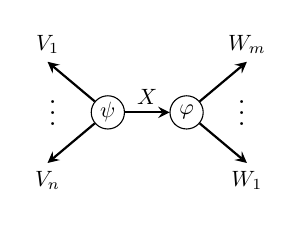
\begin{tikzpicture}
\node[morphism] (ph) at (0,0) {$\psi$};
\node[morphism] (psi) at (1,0) {$\ph$};
\node at (-0.7,0.1) {$\vdots$};
\node at (1.7,0.1) {$\vdots$};
\draw[->] (ph)-- +(220:1cm) node[pos=1.0,below,scale=0.8]
{$V_n$};
\draw[->] (ph)-- +(140:1cm) node[pos=1.0,above,scale=0.8]
{$V_1$};
\draw[->] (psi)-- +(40:1cm) node[pos=1.0,above,scale=0.8]
{$W_m$};
\draw[->] (psi)-- +(-40:1cm) node[pos=1.0,below,scale=0.8]
{$W_1$};
\draw[->] (ph) -- (psi) node[pos=0.5,above,scale=0.8] {$X$};
\end{tikzpicture}
%%%%%%%%
=
%%%%%%%%
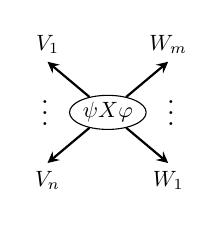
\begin{tikzpicture}
\node[ellipse, thin, scale=0.8, inner sep=1pt, draw] (ph) at (0,0)
             {$\psi\cc{X}\ph$};
\node at (-0.8,0.1) {$\vdots$};
\node at (0.8,0.1) {$\vdots$};
\draw[->] (ph)-- +(220:1cm) node[pos=1.0,below,scale=0.8] {$V_n$};
\draw[->] (ph)-- +(140:1cm) node[pos=1.0,above,scale=0.8] {$V_1$};
\draw[->] (ph)-- +(40:1cm) node[pos=1.0,above,scale=0.8]  {$W_m$};
\draw[->] (ph)-- +(-40:1cm) node[pos=1.0,below,scale=0.8] {$W_1$};
\end{tikzpicture}
%%%%%%%%%
$$
\\
$$
%%%%%%%%%
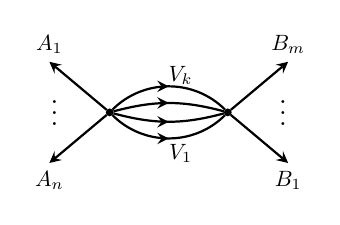
\begin{tikzpicture}
\node[dotnode] (ph) at (0,0) {};
\node[dotnode] (psi) at (1.5,0) {};
\node at (-0.7,0.1) {$\vdots$};
\node at (2.2,0.1) {$\vdots$};
\draw[->] (ph)-- +(220:1cm) node[pos=1.0,below,scale=0.8] {$A_n$};
\draw[->] (ph)-- +(140:1cm) node[pos=1.0,above,scale=0.8] {$A_1$};
\draw[->] (psi)-- +(40:1cm) node[pos=1.0,above,scale=0.8] {$B_m$};
\draw[->] (psi)-- +(-40:1cm) node[pos=1.0,below,scale=0.8] {$B_1$};
\draw[out=45,in=135, midarrow] (ph) to (psi)
                node[above,xshift=-0.6cm, yshift=0.25cm, scale=0.8] {$V_k$};
\draw[ out=15,in=165, midarrow] (ph) to (psi);
\draw[ out=-15,in=195, midarrow] (ph) to (psi);
\draw[ out=-45,in=225, midarrow] (ph) to (psi) node[below, xshift=-0.6cm, yshift=-0.3cm, scale=0.8] {$V_1$};
\end{tikzpicture}
%%%%%%%%%%%
=
%%%%%%%%%%%
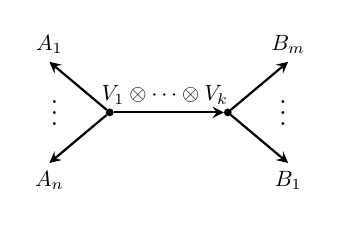
\begin{tikzpicture}
\node[dotnode] (ph) at (0,0) {};
\node[dotnode] (psi) at (1.5,0) {};
\node at (-0.7,0.1) {$\vdots$};
\node at (2.2,0.1) {$\vdots$};
\draw[->] (ph)-- +(220:1cm) node[pos=1.0,below,scale=0.8] {$A_n$};
\draw[->] (ph)-- +(140:1cm) node[pos=1.0,above,scale=0.8] {$A_1$};
\draw[->] (psi)-- +(40:1cm) node[pos=1.0,above,scale=0.8] {$B_m$};
\draw[->] (psi)-- +(-40:1cm) node[pos=1.0,below,scale=0.8] {$B_1$};
\draw[ ->] (ph) to (psi)
            node[above,xshift=-0.8cm,scale=0.8] {$V_1\otimes \dots\otimes V_k$};
\end{tikzpicture}
%%%%%%%
\qquad k\ge 0
$$
\\
$$
%%%%%%%
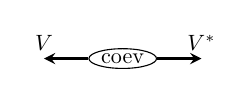
\begin{tikzpicture}
\node[ellipse, scale=0.8, inner sep=1pt, draw,thin] (ph) at (0,0)
{$\coev$};
\draw[->] (ph)-- +(180:1cm) node[pos=1.0,above,scale=0.8] {$V$};
\draw[->] (ph)-- +(0:1cm) node[pos=1.0,above,scale=0.8] {$V^*$};
\end{tikzpicture}
%%%%%%%%
=
%%%%%%%%
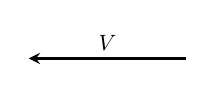
\begin{tikzpicture}
\draw[->] (2,0)-- (0,0) node[pos=0.5,above,scale=0.8] {$V$};
\end{tikzpicture}
$$
%%%%%%%%%%%%%%%%%%%%%%%%%%
\caption{Local relations for colored graphs.
%%   Here $\ph\cc{X}\psi$ denotes the morphism
%% $1 \xrightarrow{\ph \otimes \psi} 
%% V_1 \otimes \cdots \otimes V_n \otimes X \otimes X^* \otimes W_1 \otimes \cdots \otimes W_m  \xrightarrow{ev_{X^*}} 
%% V_1 \otimes \cdots \otimes V_n \otimes W_1 \otimes \cdots \otimes W_m $
%% . 
        }\label{f:local_rels1}
\end{figure}

    Local relations should be understood as follows: for any pair 
    $\Ga, \Ga'$ of colored graphs which are identical  outside a subdisk 
	$D'\subset D$, and in this disk are homeomorphic to the graphs
    shown in  \firef{f:local_rels1},  we must have $\<\Ga\>=\<\Ga'\>$. 
   \end{enumerate}

    Moreover, so defined $\<\Ga\>$ satisfies the following properties:
    \begin{enumerate} 
    \item $\<\Ga\>$ is linear in color of each vertex $v$ \textup{(}for 
         fixed colors of edges and other vertices\textup{)}.
    \item $\<\Ga\>$ is additive in colors of edges as shown in 
          \firef{f:linearity}.

\begin{figure}[ht]
$$
%%%%%%%%%%%%
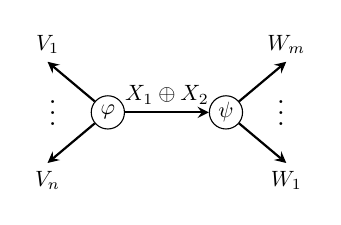
\begin{tikzpicture}
\node[morphism] (ph) at (0,0) {$\ph$};
\node[morphism] (psi) at (1.5,0) {$\psi$};
\node at (-0.7,0.1) {$\vdots$};
\node at (2.2,0.1) {$\vdots$};
\draw[->] (ph)-- +(220:1cm) node[pos=1.0,below,scale=0.8] {$V_n$};
\draw[->] (ph)-- +(140:1cm) node[pos=1.0,above,scale=0.8] {$V_1$};
\draw[->] (psi)-- +(40:1cm) node[pos=1.0,above,scale=0.8] {$W_m$};
\draw[->] (psi)-- +(-40:1cm) node[pos=1.0,below,scale=0.8] {$W_1$};
\draw[->] (ph) -- (psi) node[pos=0.5,above,scale=0.8] {$X_1\oplus X_2$};
\end{tikzpicture}
%%%%%%%%%%%%
=
%%%%%%%%%%%%
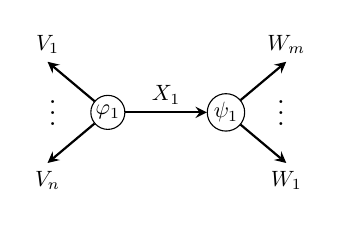
\begin{tikzpicture}
\node[morphism] (ph) at (0,0) {$\ph_1$};
\node[morphism] (psi) at (1.5,0) {$\psi_1$};
\node at (-0.7,0.1) {$\vdots$};
\node at (2.2,0.1) {$\vdots$};
\draw[->] (ph)-- +(220:1cm) node[pos=1.0,below,scale=0.8]{$V_n$};
\draw[->] (ph)-- +(140:1cm) node[pos=1.0,above,scale=0.8]{$V_1$};
\draw[->] (psi)-- +(40:1cm) node[pos=1.0,above,scale=0.8]{$W_m$};
\draw[->] (psi)-- +(-40:1cm) node[pos=1.0,below,scale=0.8]{$W_1$};
\draw[->] (ph) -- (psi) node[pos=0.5,above,scale=0.8] {$X_1$};
\end{tikzpicture}
%%%%%%%%%%%%
+
%%%%%%%%%%%%
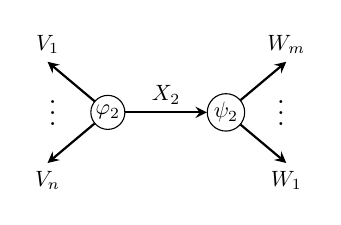
\begin{tikzpicture}
\node[morphism] (ph) at (0,0) {$\ph_2$};
\node[morphism] (psi) at (1.5,0) {$\psi_2$};
\node at (-0.7,0.1) {$\vdots$};
\node at (2.2,0.1) {$\vdots$};
\draw[->] (ph)-- +(220:1cm) node[pos=1.0,below,scale=0.8]{$V_n$};
\draw[->] (ph)-- +(140:1cm) node[pos=1.0,above,scale=0.8]{$V_1$};
\draw[->] (psi)-- +(40:1cm) node[pos=1.0,above,scale=0.8]{$W_m$};
\draw[->] (psi)-- +(-40:1cm) node[pos=1.0,below,scale=0.8]{$W_1$};
\draw[->] (ph) -- (psi) node[pos=0.5,above,scale=0.8] {$X_2$};
\end{tikzpicture}
%%%%%%%%%%%%
$$
\caption{Linearity of $\<\Ga\>$. Here $\ph_1,\ph_2$ are compositions
of $\ph$ with projector $X_1\oplus X_2\to X_1$ (respectively, 
$X_1\oplus X_2\to X_2$), and similarly for $\psi_1,\psi_2$.
}\label{f:linearity}
\end{figure}
    \item If $\Ga,\Ga'$ are two isomorphic colorings of the same graph,
      then $\<\Ga\>=\<\Ga'\>$. 
    
    \item Composition property: if $D'\subset D$ is a subdisk such
      that $\del D'$ does not contain vertices of $\Ga$ and meets edges of
      $\Ga$ transversally, then   $\<\Ga\>_D$ will not change if we replace
      subgraph $\Ga\cap D'$ by a single vertex colored by
      $\<\Ga\cap D'\>_{D'}$.

  \end{enumerate}
The vector $\<\Ga\>$ is called the {\em evaluation} of $\Ga$.
\end{thrm}

To define local relations between embedded graphs, Kirillov defines the space of null graphs as follows. Let
$\Ga=c_1\Ga_1+\dots+c_n\Ga_n$ be a formal linear
combination of colored graphs in $\Si$.  If there exists an embedded disk $D \subset M$ such that
\begin{enumerate}
  \item $\Ga$ is transversal to $\del D$ (i.e., no vertices of $\Ga_i$ 
      are on the boundary of $D$ and edges of each $\Ga_i$ meet 
      $\del D$ transversally),
  \item all $\Ga_i$ coincide outside of $D$,
  \item and $\<\Ga\>_D=\sum c_i\<\Ga_i\cap D\>_D=0$;
\end{enumerate}
then $\Ga$ is called a null graph. 




\begin{defn}
The vector space $H := \Hs(\Si, \VV)$ associated to a oriented surface $\Si$ with boundary condition $\VV$ by the spherical fusion category $\mathcal A$ is the quotient space
 $$
   \Hs(\Si, \VV)=\VGr(\Si, \VV)/N(\Si, \VV)
  $$
  where $N(\Si, \VV)$ is  the subspace spanned by null graphs 
  (for all possible embedded disks  $D \subset \Si$). 
\end{defn}
%% The action of the mapping class group on H


%% TODO: \subsection{Birman's mapping class group generators}




\subsection{Strictification}
The colored graph construction takes a strict pivotal category as input, so we must strictify $\Vect_G^\omega$ to get an equivalent strict pivotal monoidal $\widehat \vgo$. Every pivotal category is equivalent to a strict pivotal monoidal category by first strictifying with respect to the monoidal structure, and then strictifying with respect to the pivotal structure as follows \cite{ns}.

Given a monoidal category $\mC$, there exists a monoidally equivalent strict monoidal category $\mC'$ with objects consisting of all finite lists of objects of $\mC$ and morphisms defined by
\begin{align*}
& \Hom_{\mC'}([A_1, \ldots, A_n], [B_1, \ldots, B_m]) = \\
& \qquad \Hom_\mC(((\cdots((A_1 \otimes A_2) \otimes A_3) \otimes \cdots \otimes A_n, ((\cdots((B_1 \otimes B_2) \otimes B_3) \otimes \cdots \otimes B_m).
\end{align*}

The tensor product in $\mC'$ is concatenation of lists. The strictification functor applies the obvious unique composition of associators to both objects and morphisms of $\mC$, and the coherence map does the same. If $\mC$ is pivotal, this monoidal equivalence extends to an equivalence of pivotal monoidal categories (where the pivotal structure on $\mC'$ is given by applying the strictification functor to the pivotal structure of $\mC$).

Given a pivotal strict monoidal category $\mC'$, there is a strict pivotal monoidal category $\widehat \mC$ equivalent, as a pivotal monoidal category, to $\mC'$.  The objects of $\widehat \mC$ are pairs $(X, \epsilon)$ for which there exists $r \in \NN_0$ such that $X \in \mC^r$ and $\epsilon \in \ZZ_2^r$. The morphisms are
$$\Hom_{\widehat \mC}((X, \epsilon), (Y, \epsilon)) = \Hom_{\mC'}(X_1^{\epsilon_1} \otimes \cdots \otimes X_r^{\epsilon_r}, Y_1^{\epsilon_1} \otimes \cdots \otimes Y_s^{\epsilon_s}),$$
where $X^\epsilon$ is defined by $X^0 = X$ and $X^1 = X^*$. The tensor product is given by concatenation. The duality functor on $\widehat \mC$ is given by
$$(X, \epsilon)^* = ((X_r, \ldots, X_1), (\epsilon_r + 1, \ldots, \epsilon_1 + 1)).$$
The evaluation function $\ev_{(X, \epsilon)}$ on $\widehat \mC$ is inductively defined using tensor products of identities, $j_{X_i}$'s, and evaluation maps $\ev_{X_i}$ in $\mC'$, and similarly for coevaluation.  This strictification functor maps $X \in \mC'$ to $(X, 0)$ and acts on morphisms as the identity.  The coherence maps are also identity maps.

Slightly abusing notation, we will sometimes use the same symbol for both $X \in \mC$ and its images in $\mC'$ and $\widehat \mC$ under the strictification functors.


%%%%%%%%%%%%%%%%%%%%%%%%%%%%%%%%%%%%%%%%%%%%%%%%%%%%
%
%  New template code for TAMU Theses and Dissertations starting Fall 2016.  
%
%
%  Author: Sean Zachary Roberson
%  Version 3.17.09
%  Last Updated: 9/21/2017
%
%%%%%%%%%%%%%%%%%%%%%%%%%%%%%%%%%%%%%%%%%%%%%%%%%%%

%%%%%%%%%%%%%%%%%%%%%%%%%%%%%%%%%%%%%%%%%%%%%%%%%%%%%%%%%%%%%%%%%%%%%%%
%%%                           SECTION II
%%%%%%%%%%%%%%%%%%%%%%%%%%%%%%%%%%%%%%%%%%%%%%%%%%%%%%%%%%%%%%%%%%%%%%


\chapter{PAGES WITH A FIGURE, A TABLE AND AN EQUATION}
\section{Figures: Placement, Size, and Captions}
This is a figure template.
\begin{figure}[ht]
\centering
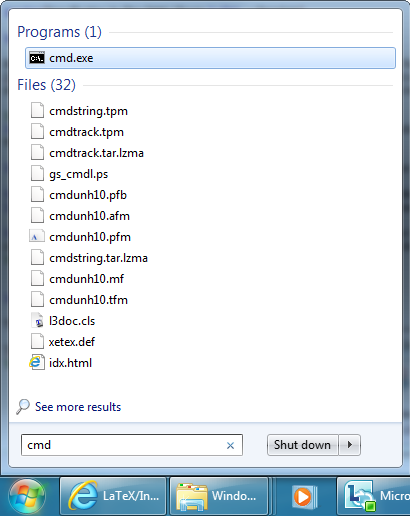
\includegraphics[scale=0.75]{TAMUthesis_CMD_windows.png}
\caption[The command line compiler in Windows.]{The command line compiler in Windows. It is not suggested that you compile using this method. See compilation instructions in the README.}

\label{fig:CMD_1}

\end{figure}

Figure (and table) titles should be consistent through the document. All captions should be placed either above or below the object it describes. This is done by placing the \textit{caption} in the correct place. While continued figures are allowed by the Thesis Manual, it is not suggested that any continued figures be included in a \LaTeX\ document. The figure below is from Linux Mint, showing a portion of a desktop.

\begin{figure}[H]
	\centering
	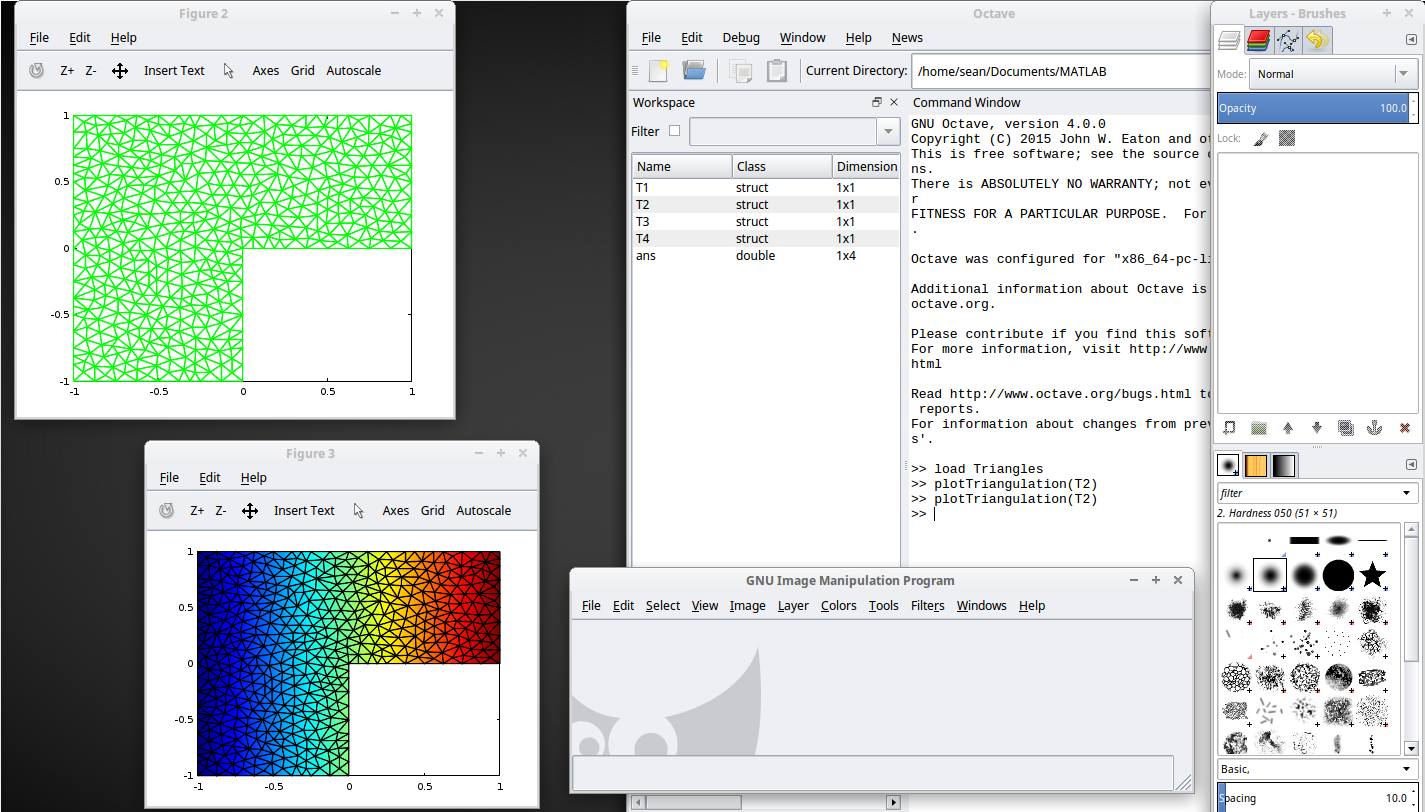
\includegraphics[width = 5.75in]{Desktop.png}
	\caption{A typical desktop space in Linux Mint.}
\end{figure}

The figure below is taken from R. While there are packages available to import graphics from R, MATLAB, and similar software, it is probably best to export plots generated by these programs as a PNG file, and then import it via the \textit{includegraphics} command.

\begin{figure}[H]
	\centering
	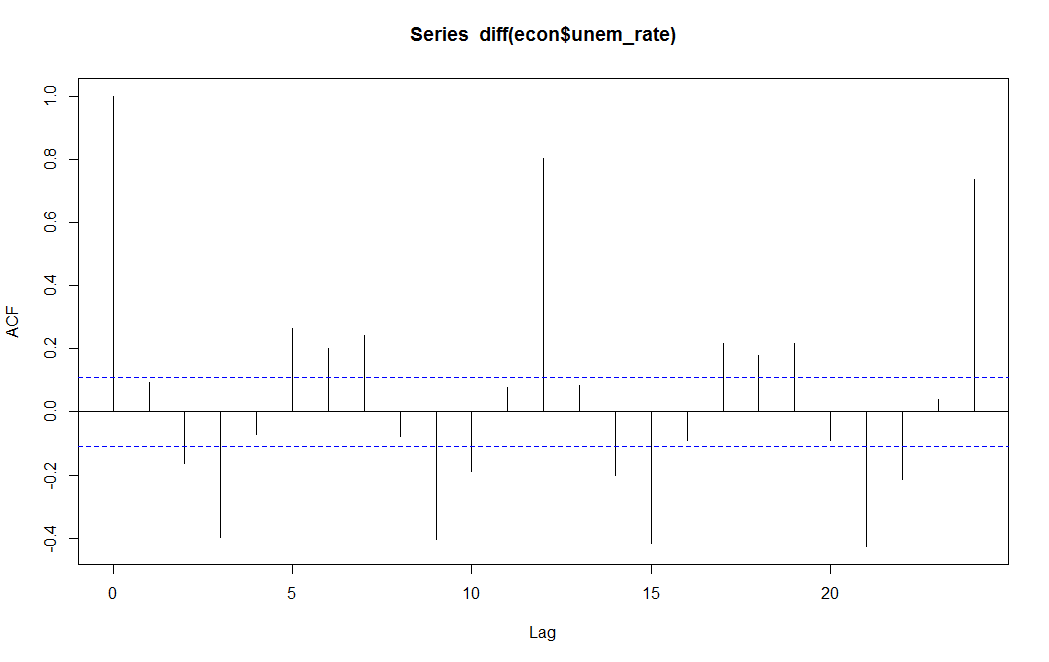
\includegraphics[scale=0.55]{UnemDiffACF.png}
	\singlespace
	\caption{The autocorrelation function (ACF) of the differenced unemployment series. Seasonal adjustments may be needed.}
\end{figure}

It is highly suggested that you scale the figures so that they fit within the margins. Almost all the figures included in this document for the sake of example have been scaled. It is best to use PNG and JPEG files as figures.

The last figure here is a screenshot from the Linux terminal.

\begin{figure}[H]
	\centering
	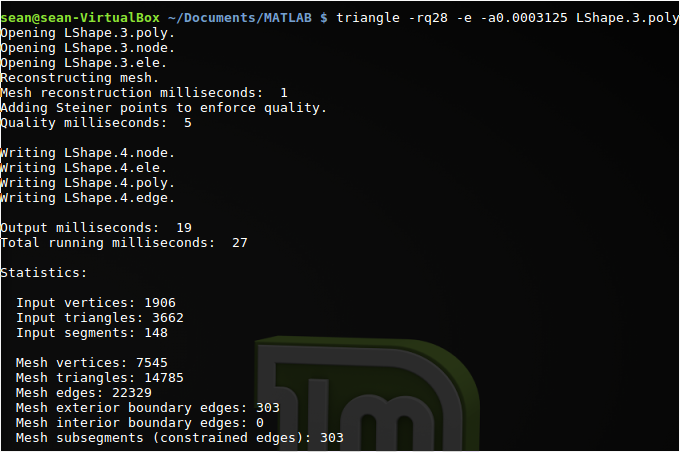
\includegraphics[width=4.75in]{Terminal1.png}
	\caption{The Linux terminal. The commands shown are from a two-dimensional mesh generator that triangulates a domain in the plane. Files containing nodes, elements, the polygon, and the edges are created.}
\end{figure}

\section{Table Placement, Size and Table Title}

Here is a table, displaying band and auxiliary scores from the 2011 Arcadia Festival of Bands held in Arcadia, CA \cite{ARCADIA}.

\begin{table}[h!]
	\centering

	\label{Band}
	\begin{tabular}{|l|l|l|}
		\hline
		School Name & Band Score & Auxiliary Score \\ \hline
		Rancho Bernardo & 96.15 & 89.15 \\ \hline
		Mt. Carmel & 95.30 & 83.55 \\ \hline
		Riverside King & 93.85 & 91.75 \\ \hline
		Diamond Bar & 93.20 & 88.60 \\ \hline
		El Dorado & 92.80 & 95.45 \\ \hline
		Chino & 92.65 & 91.45 \\ \hline
		Henry J. Kaiser & 92.60 & 87.55 \\ \hline
		Glendora & 92.60 & 89.15 \\ \hline
		Montebello & 90.50 & 82.70 \\ \hline
		Mira Mesa & 89.65 & 91.50 \\ \hline
	\end{tabular}
	\caption{Scores from the 2011 Arcadia Festival of Bands.}
\end{table}

The table is sorted by band score. There is more text here to demonstrate how the template handles spacing between tables and body text. Also note how the table caption is in a smaller font size than the body text.

\section{Equations}

The following format is recommended to be used to display equations.

%Make other examples.
\begin{equation} \label{Equ.2.1}
y=c_1\cos(t)+c_2\sin(t)
\end{equation}
\begin{equation} \label{Equ.2.2}
e^{it}=\cos(t)+i\sin(t)
\end{equation}

Equation \ref{Equ.2.1} is the general solution to the differential equation $y''+y=0$. In the source code, the \textit{ref} command allows you to refer to an equation by a label you created. References must be made after the equation has been created; attempting to refer to an equation before it is defined results in a question mark placeholder. Some more sample equations are below. Notice the first set below is not numbered.
%%
\begin{align*}
\log (x^n) &= \log (x \cdot x \cdot \ldots \cdot x) \\
&= \log x + \log x + \ldots + \log x \\
&= n \log x
\end{align*}
\begin{equation} \label{Equ.2.3}
X^T X \mathbf{u} = X^T \mathbf{y}
\end{equation}
\begin{equation}\label{Equ.2.4}
u(x, t) = \int_{-\infty}^{\infty} G(x, \tau) \exp\left(-\frac{(t-\tau)^2}{4kt}\right) \ d\tau
\end{equation}
\begin{gather}
\mathcal{L}(f) = \int_{0}^{\infty} e^{-st} f(t) \ dt \\
\begin{split} \label{Equ.2.5}
\mathcal{F}(f) = \frac{1}{2\pi}\int_{-\infty}^{\infty} e^{i \omega x} f(x) \ dx
\end{split}
\end{gather}

You can use labels to refer to equations you create. \ref{Equ.2.5} is the \textbf{Laplace transform} used extensively in differential equations. \ref{Equ.2.3} is the matrix representation of the \textbf{normal equations} used in least-squares regression.

To have equations without labels appearing the right margin, simply add an asterisk to the name of the environment (equation, align, etc.) when making the declaration.


\section{Theorems and Proofs: Examples}

This section will show an example usage of the theorem and proof environments, typically used for mathematics students. To use these environments, you must have the package \textbf{amsthm} declared in the preamble of your document. For this template, this is already declared in the main file. You may choose to remove this declaration if your document will not make use of theorems and proofs.

Theorems can be numbered, as the one below is, or you can force a different label to appear. For example, you can state the Bolzano-Weierstass theorem and have the names appear as the theorem label. See the examples below.

Sometimes you may have a theorem with multiple parts or multiple conditions. You can use other list environments, such as enumerate, inside the theorem environment declared to list these conditions. The final example at the end of this block shows this with the Invertible Matrix Theorem, which has several equivalent statements.

\newtheorem{thm}{Theorem}
\begin{thm}
	Suppose $f$ is of class $\mathcal{C}^1$ and $g$ is of class $\mathcal{C}^2$, and that the compact set $D$ and its boundary satisfy the hypotheses of Green's Theorem.  Then
	\[ \iint \limits_D f\nabla^2 g \ dA = \oint_{\partial D} f(\nabla g) \cdot \mathbf{n} \ ds - \iint \limits_D \nabla f \cdot \nabla g \ dA . \]
\end{thm}

\begin{proof}
	Begin with the integral of $f\nabla g \cdot n$ taken over the boundary of D.  By the second vector form of Green's Theorem,
	\begin{align*}
	\oint_{\partial D} f\nabla g \cdot n \ ds &= \iint \limits_D \nabla \cdot (f\nabla g) \ dA \\
	&= \iint \limits_D f\nabla^2 g + \nabla f \cdot \nabla g \ dA.
	\end{align*}
	
	Rearranging yields the desired.
\end{proof}

\begin{thm}[Bolzano-Weierstrass]
	Every bounded real sequence has a convergent subsequence.
\end{thm}

\begin{thm}[Invertible Matrix Theorem\footnote{This is an incomplete list.}]
	For any square matrix $A$ with $n$ rows and columns, the following are equivalent.
	\begin{enumerate}
		\item $A$ is invertible.
		\item The equation $A\mathbf{x}=\mathbf{0}$ has only the trivial solution $\mathbf{x} = \mathbf{0}.$
		\item For any nonzero $\mathbf{b}, \ A\mathbf{x} = \mathbf{b}$ has exactly one solution.
		\item The columns of $A$ form a linearly independent set.
		\item Zero is not an eigenvalue of $A$.
		\item $A$ has full rank.
		\item The determinant of $A$ is not zero.
	\end{enumerate}
\end{thm}

There is currently no set format on how propositions and theorems should be laid out in the document. The idea is to remain consistent. It is best to not customize the appearance of theorems so that they can easily be distinguished from body text - just like figures, tables, and headings.

\section{Another Table Example}
For the sake of testing the appearance of the list of tables, a second table will be displayed here. This table displays a list of some major universities and their enrollments during fall 2015. This table is sorted in descending order of enrollment.
%The savenotes environment, loaded from the footnote package
%(which in turn is loaded from mdwtools)
%allows you to use footnotes in tables, if needed.
\begin{savenotes}
\begin{table}[h!]
	\centering
	\label{my-label}
	\begin{tabular}{|l|l|l|}
		\hline
		School & City and State & Fall 2015 Enrollment  \\ \hline
		Texas A\&M University\footnote{Gig 'em!} & College Station, TX & 64,376  \\ \hline
		Ohio State University\footnote{This number describes enrollments at the Columbus campus; enrollments at regional campuses in Lima, Mansfield, Marion, Newark, and Wooster are not counted.} & Columbus, OH & 58,322 \\ \hline
		Iowa State University & Ames, IA & 36,001 \\ \hline
		University of California, San Diego & La Jolla, CA & 33,735   \\ \hline
		University of West Florida & Pensacola, FL & 12,798 \\ \hline
		Massachusetts Institute of Technology & Cambridge, MA & 11,319   \\ \hline
	\end{tabular}
	\caption{Some major universities and their fall 2015 enrollments.}
\end{table}
\end{savenotes}

Naturally, tables and footnotes do not go together. If you attempted to write a footnote inside a table, there will be nothing at the bottom of the page, yet the footnote marker will still appear. To remedy this, the \textit{footnote} package has been loaded from the \textit{mdwtools} package. Check your TeX distribution to see if \textit{mdwtools} is installed. See the source code for how this is implemented.

Here are some blank floats.

\begin{figure}[!h]
	\caption{A blank float.}
\end{figure}

\begin{figure}[!h]
	\caption{Another blank float.}
\end{figure}
%%%%%%%%%%%%%%%%%%%%%%%%%%%%%%%%%%%%%%%%%%%%%%%%%%%
%
%  New template code for TAMU Theses and Dissertations starting Fall 2016.  
%
%
%  Author: Sean Zachary Roberson
%  Version 3.17.09
%  Last Updated: 9/21/2017
%
%%%%%%%%%%%%%%%%%%%%%%%%%%%%%%%%%%%%%%%%%%%%%%%%%%%

%%%%%%%%%%%%%%%%%%%%%%%%%%%%%%%%%%%%%%%%%%%%%%%%%%%%%%%%%%%%%%%%%%%%%%%
%%%                           SECTION II
%%%%%%%%%%%%%%%%%%%%%%%%%%%%%%%%%%%%%%%%%%%%%%%%%%%%%%%%%%%%%%%%%%%%%%


\chapter{PAGES WITH A FIGURE, A TABLE AND AN EQUATION}
\section{Figures: Placement, Size, and Captions}
This is a figure template.
\begin{figure}[ht]
\centering
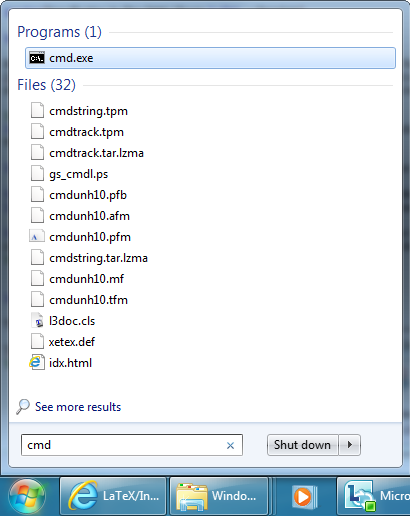
\includegraphics[scale=0.75]{TAMUthesis_CMD_windows.png}
\caption[The command line compiler in Windows.]{The command line compiler in Windows. It is not suggested that you compile using this method. See compilation instructions in the README.}

\label{fig:CMD_1}

\end{figure}

Figure (and table) titles should be consistent through the document. All captions should be placed either above or below the object it describes. This is done by placing the \textit{caption} in the correct place. While continued figures are allowed by the Thesis Manual, it is not suggested that any continued figures be included in a \LaTeX\ document. The figure below is from Linux Mint, showing a portion of a desktop.

\begin{figure}[H]
	\centering
	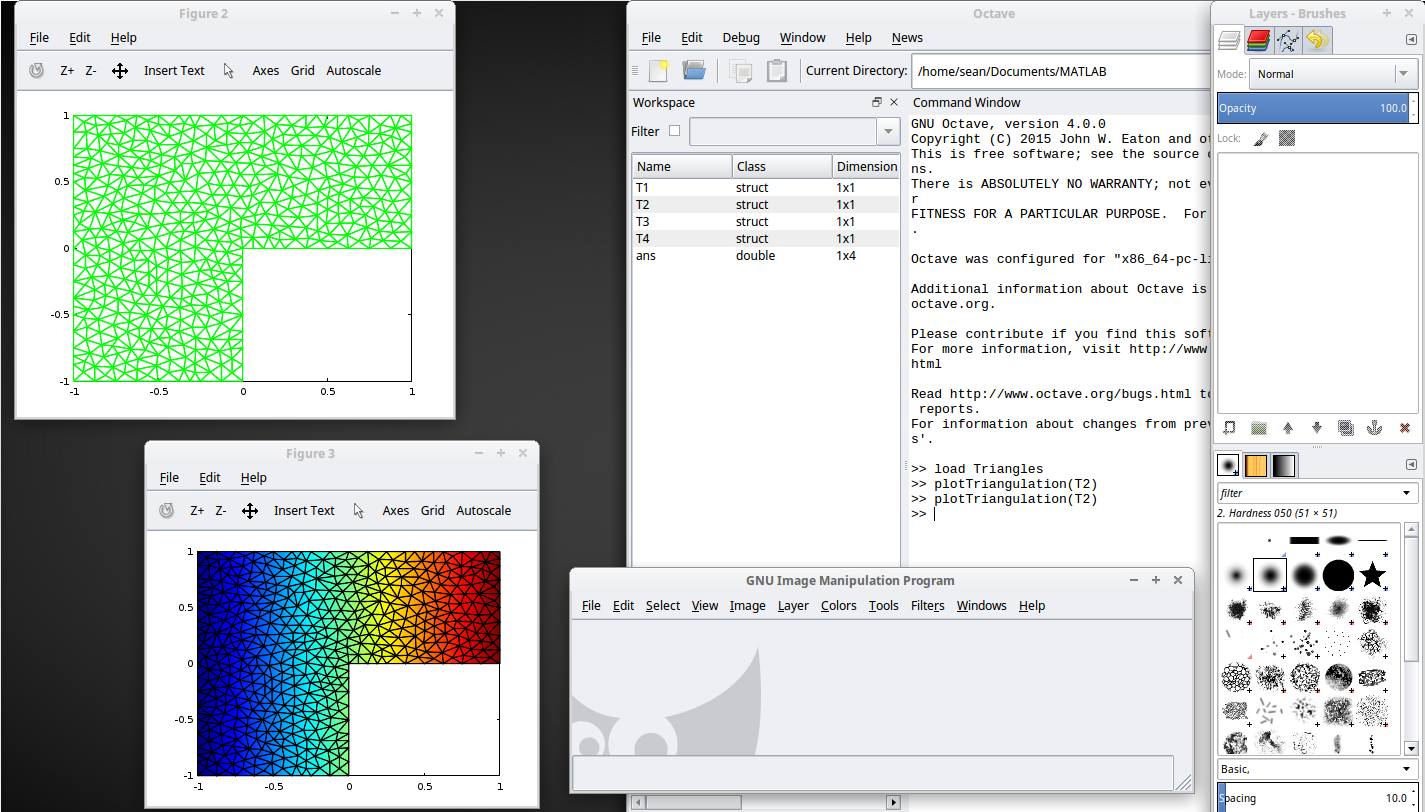
\includegraphics[width = 5.75in]{Desktop.png}
	\caption{A typical desktop space in Linux Mint.}
\end{figure}

The figure below is taken from R. While there are packages available to import graphics from R, MATLAB, and similar software, it is probably best to export plots generated by these programs as a PNG file, and then import it via the \textit{includegraphics} command.

\begin{figure}[H]
	\centering
	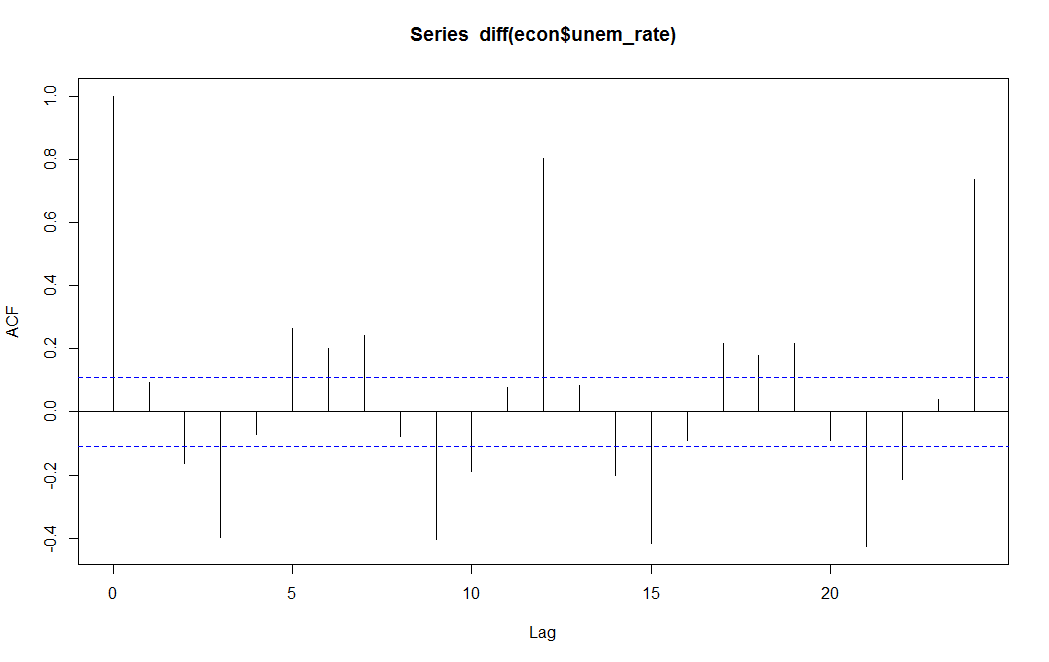
\includegraphics[scale=0.55]{UnemDiffACF.png}
	\singlespace
	\caption{The autocorrelation function (ACF) of the differenced unemployment series. Seasonal adjustments may be needed.}
\end{figure}

It is highly suggested that you scale the figures so that they fit within the margins. Almost all the figures included in this document for the sake of example have been scaled. It is best to use PNG and JPEG files as figures.

The last figure here is a screenshot from the Linux terminal.

\begin{figure}[H]
	\centering
	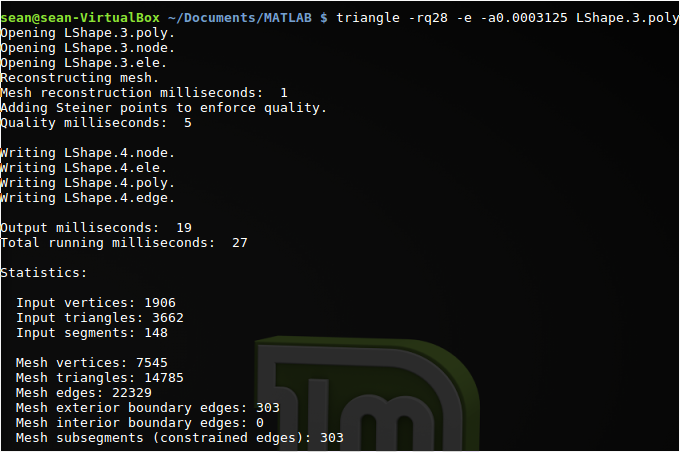
\includegraphics[width=4.75in]{Terminal1.png}
	\caption{The Linux terminal. The commands shown are from a two-dimensional mesh generator that triangulates a domain in the plane. Files containing nodes, elements, the polygon, and the edges are created.}
\end{figure}

\section{Table Placement, Size and Table Title}

Here is a table, displaying band and auxiliary scores from the 2011 Arcadia Festival of Bands held in Arcadia, CA \cite{ARCADIA}.

\begin{table}[h!]
	\centering

	\label{Band}
	\begin{tabular}{|l|l|l|}
		\hline
		School Name & Band Score & Auxiliary Score \\ \hline
		Rancho Bernardo & 96.15 & 89.15 \\ \hline
		Mt. Carmel & 95.30 & 83.55 \\ \hline
		Riverside King & 93.85 & 91.75 \\ \hline
		Diamond Bar & 93.20 & 88.60 \\ \hline
		El Dorado & 92.80 & 95.45 \\ \hline
		Chino & 92.65 & 91.45 \\ \hline
		Henry J. Kaiser & 92.60 & 87.55 \\ \hline
		Glendora & 92.60 & 89.15 \\ \hline
		Montebello & 90.50 & 82.70 \\ \hline
		Mira Mesa & 89.65 & 91.50 \\ \hline
	\end{tabular}
	\caption{Scores from the 2011 Arcadia Festival of Bands.}
\end{table}

The table is sorted by band score. There is more text here to demonstrate how the template handles spacing between tables and body text. Also note how the table caption is in a smaller font size than the body text.

\section{Equations}

The following format is recommended to be used to display equations.

%Make other examples.
\begin{equation} \label{Equ.2.1}
y=c_1\cos(t)+c_2\sin(t)
\end{equation}
\begin{equation} \label{Equ.2.2}
e^{it}=\cos(t)+i\sin(t)
\end{equation}

Equation \ref{Equ.2.1} is the general solution to the differential equation $y''+y=0$. In the source code, the \textit{ref} command allows you to refer to an equation by a label you created. References must be made after the equation has been created; attempting to refer to an equation before it is defined results in a question mark placeholder. Some more sample equations are below. Notice the first set below is not numbered.
%%
\begin{align*}
\log (x^n) &= \log (x \cdot x \cdot \ldots \cdot x) \\
&= \log x + \log x + \ldots + \log x \\
&= n \log x
\end{align*}
\begin{equation} \label{Equ.2.3}
X^T X \mathbf{u} = X^T \mathbf{y}
\end{equation}
\begin{equation}\label{Equ.2.4}
u(x, t) = \int_{-\infty}^{\infty} G(x, \tau) \exp\left(-\frac{(t-\tau)^2}{4kt}\right) \ d\tau
\end{equation}
\begin{gather}
\mathcal{L}(f) = \int_{0}^{\infty} e^{-st} f(t) \ dt \\
\begin{split} \label{Equ.2.5}
\mathcal{F}(f) = \frac{1}{2\pi}\int_{-\infty}^{\infty} e^{i \omega x} f(x) \ dx
\end{split}
\end{gather}

You can use labels to refer to equations you create. \ref{Equ.2.5} is the \textbf{Laplace transform} used extensively in differential equations. \ref{Equ.2.3} is the matrix representation of the \textbf{normal equations} used in least-squares regression.

To have equations without labels appearing the right margin, simply add an asterisk to the name of the environment (equation, align, etc.) when making the declaration.


\section{Theorems and Proofs: Examples}

This section will show an example usage of the theorem and proof environments, typically used for mathematics students. To use these environments, you must have the package \textbf{amsthm} declared in the preamble of your document. For this template, this is already declared in the main file. You may choose to remove this declaration if your document will not make use of theorems and proofs.

Theorems can be numbered, as the one below is, or you can force a different label to appear. For example, you can state the Bolzano-Weierstass theorem and have the names appear as the theorem label. See the examples below.

Sometimes you may have a theorem with multiple parts or multiple conditions. You can use other list environments, such as enumerate, inside the theorem environment declared to list these conditions. The final example at the end of this block shows this with the Invertible Matrix Theorem, which has several equivalent statements.

\newtheorem{thm}{Theorem}
\begin{thm}
	Suppose $f$ is of class $\mathcal{C}^1$ and $g$ is of class $\mathcal{C}^2$, and that the compact set $D$ and its boundary satisfy the hypotheses of Green's Theorem.  Then
	\[ \iint \limits_D f\nabla^2 g \ dA = \oint_{\partial D} f(\nabla g) \cdot \mathbf{n} \ ds - \iint \limits_D \nabla f \cdot \nabla g \ dA . \]
\end{thm}

\begin{proof}
	Begin with the integral of $f\nabla g \cdot n$ taken over the boundary of D.  By the second vector form of Green's Theorem,
	\begin{align*}
	\oint_{\partial D} f\nabla g \cdot n \ ds &= \iint \limits_D \nabla \cdot (f\nabla g) \ dA \\
	&= \iint \limits_D f\nabla^2 g + \nabla f \cdot \nabla g \ dA.
	\end{align*}
	
	Rearranging yields the desired.
\end{proof}

\begin{thm}[Bolzano-Weierstrass]
	Every bounded real sequence has a convergent subsequence.
\end{thm}

\begin{thm}[Invertible Matrix Theorem\footnote{This is an incomplete list.}]
	For any square matrix $A$ with $n$ rows and columns, the following are equivalent.
	\begin{enumerate}
		\item $A$ is invertible.
		\item The equation $A\mathbf{x}=\mathbf{0}$ has only the trivial solution $\mathbf{x} = \mathbf{0}.$
		\item For any nonzero $\mathbf{b}, \ A\mathbf{x} = \mathbf{b}$ has exactly one solution.
		\item The columns of $A$ form a linearly independent set.
		\item Zero is not an eigenvalue of $A$.
		\item $A$ has full rank.
		\item The determinant of $A$ is not zero.
	\end{enumerate}
\end{thm}

There is currently no set format on how propositions and theorems should be laid out in the document. The idea is to remain consistent. It is best to not customize the appearance of theorems so that they can easily be distinguished from body text - just like figures, tables, and headings.

\section{Another Table Example}
For the sake of testing the appearance of the list of tables, a second table will be displayed here. This table displays a list of some major universities and their enrollments during fall 2015. This table is sorted in descending order of enrollment.
%The savenotes environment, loaded from the footnote package
%(which in turn is loaded from mdwtools)
%allows you to use footnotes in tables, if needed.
\begin{savenotes}
\begin{table}[h!]
	\centering
	\label{my-label}
	\begin{tabular}{|l|l|l|}
		\hline
		School & City and State & Fall 2015 Enrollment  \\ \hline
		Texas A\&M University\footnote{Gig 'em!} & College Station, TX & 64,376  \\ \hline
		Ohio State University\footnote{This number describes enrollments at the Columbus campus; enrollments at regional campuses in Lima, Mansfield, Marion, Newark, and Wooster are not counted.} & Columbus, OH & 58,322 \\ \hline
		Iowa State University & Ames, IA & 36,001 \\ \hline
		University of California, San Diego & La Jolla, CA & 33,735   \\ \hline
		University of West Florida & Pensacola, FL & 12,798 \\ \hline
		Massachusetts Institute of Technology & Cambridge, MA & 11,319   \\ \hline
	\end{tabular}
	\caption{Some major universities and their fall 2015 enrollments.}
\end{table}
\end{savenotes}

Naturally, tables and footnotes do not go together. If you attempted to write a footnote inside a table, there will be nothing at the bottom of the page, yet the footnote marker will still appear. To remedy this, the \textit{footnote} package has been loaded from the \textit{mdwtools} package. Check your TeX distribution to see if \textit{mdwtools} is installed. See the source code for how this is implemented.

Here are some blank floats.

\begin{figure}[!h]
	\caption{A blank float.}
\end{figure}

\begin{figure}[!h]
	\caption{Another blank float.}
\end{figure}
%%%%%%%%%%%%%%%%%%%%%%%%%%%%%%%%%%%%%%%%%%%%%%%%%%%
%
%  New template code for TAMU Theses and Dissertations starting Fall 2016.  
%
%
%  Author: Sean Zachary Roberson
%  Version 3.17.09
%  Last Updated: 9/21/2017
%
%%%%%%%%%%%%%%%%%%%%%%%%%%%%%%%%%%%%%%%%%%%%%%%%%%%
%%%%%%%%%%%%%%%%%%%%%%%%%%%%%%%%%%%%%%%%%%%%%%%%%%%%%%%%%%%%%%%%%%%%%%
%%                           SECTION III
%%%%%%%%%%%%%%%%%%%%%%%%%%%%%%%%%%%%%%%%%%%%%%%%%%%%%%%%%%%%%%%%%%%%%



\chapter{RESULTS}


%% \begin{prop}
%% The action of the mapping class group on the vector space $H$ induced by the action of the orientation-preserving homeomorphisms on the surface $\Si$ is well-defined.
%% \end{prop}
%% \begin{proof}
%% The orientation-preserving group $\Homeo^+(M)$ acts on colored embedded graphs in $\Si$.  To see that the mapping class group $\MCG(\Si)$ has a well-defined action on $H$, we need to check two things: first, that isotopic homeomorphisms acting on a colored graph take it to equivalent colored graphs and, second, that a homeomorphism maps equivalent colored graphs to equivalent colored graphs.

%% For the first, suppose $f, g \in Homeo^+(M)$ are isotopic, with $H: M \times I \to M$ an isotopy from $f$ to $g$.  Let $i: \Gamma \to M$ be an graph embedding.  Then $H \circ i$ is an isotopy from $f \circ i$ to $g \circ i$.    

%% For the second,  to check that a homeomorphism $f \in \Homeo^+(M)$ preserves equivalence of colored graphs, it suffices to check that it in the case of each local move.  Since the mapping class group is generated by Dehn twists, all the local moves reduce to the isotopy move. 

%% To check that isotopic colored graphs get mapped to equivalent colored graphs, suppose $\Gamma$ is a graph and $i: \Gamma to M$ and $j: \Gamma \to M$ are isotopic embeddings. Let $H: \Gamma \times I \to M$ be an isotopy from $i$ to $j$.  Let $f \in \Homeo^+(M)$.  Then $f \circ H$ is an isotopy from $f \circ i$ to $f \circ j$.  

%% Thus, the action of the mapping class group on $H$ is well-defined.
%% \end{proof}

%% TODO: Prove that the Turaev-Viro/ RT construction gives the same thing for equivalent TQFTs

\newcommand{\B}{\mathcal B}

%% \begin{prop} \label{prop:equivCats}
%% Let $\Sigma$ be a compact surface with boundary. Let $\mathcal A$ and $\mathcal B$ be monoidally equivalent spherical fusion categories.  Then
%% the TVBW-representation $\rho_A : \MCG(\Sigma) \to GL(H_A)$ associated to $\mathcal A$ is isomorphic to the representation associated to $\mathcal B$.
%% \end{prop}
%% \begin{proof}
%% Let $(F, J)$ be a monoidal equivalence from $\A$ to $\B$. I claim that $F$ induces an isomorphism $\overline{F}: H_A \to H_B$ by acting on the labels.  To see that this is well-defined, we need to check that if $\phi \in \Hom(\one, V_1 \otimes \cdot \otimes V_n)$ then $F(\phi) \in    \Hom(\one, F(V_1) \otimes \cdot \otimes F(V_n))$


%% To see this, we need to check that $F$ preserves the local relations.  For the first local relation (contracting an edge), we need to check that $F(\ev_{F(X)}) \circ (F(\phi) \otimes F(\psi)) = F(\ev_{F(X)} \circ (\phi \otimes \psi))$.
%% \end{proof}


To show that the image of any $\Vect_G^\omega$ mapping class group representation is finite, we will analyze the action of the mapping class group on a finite collection of colored graphs that span the representation space $H$.  To define this spanning set, we will need the following definitions of simple morphisms and colored graphs.


\begin{defn} \label{def:simple_morphism}
  Let $g_1, \ldots, g_n \in G$ and $\epsilon_1, \ldots, \epsilon_n  \in \{\pm 1\} = \ZZ_2$.  A morphism  $\phi \in \langle (\delta_{g_1}, \epsilon_1), \ldots, (\delta_{g_n}, \epsilon_n) \rangle = \Hom_{\widehat{\vgo}}(1, (\delta_{g_1}, \epsilon_1) \otimes \cdots \otimes (\delta_{g_n}, \epsilon_n)) = \Hom_{\vgo}(1, (( \cdots ((\delta_{g_1^{\epsilon_1}} \otimes \delta_{g_2^{\epsilon_2}}) \otimes \cdots  \otimes \delta_{g_n^{\epsilon_n}})$ will be called \emph{simple} if it is the composition of the isomorphism $\one \cong \delta_1$ and  tensor product isomorphisms of the form $\delta_{gh} \cong \delta_g \otimes \delta_h$ in $\vgo$.
\end{defn}

By MacLane's coherence theorem applied to the $\vgo$ Hom-space, there is a unique simple morphism in $\langle (\delta_{g_1}, \epsilon_1), \ldots, (\delta_{g_n}, \epsilon_n) \rangle$ whenever $\prod_{i=1}^n g_i = 1$. This simple morphism is a canonical basis element for the 1-dimensional space $\langle (\delta_{g_1}, \epsilon_1), \ldots, (\delta_{g_n}, \epsilon_n) \rangle$.  We will describe a map between such spaces as multiplication by a scalar, where the scalar is the matrix coefficient of the map with respect to these canonical bases.

\begin{defn} \label{def:simple_graph}
Let $\Gamma$ be a graph embedded in a surface $\Si$.  A $\widehat {\Vect_G^\omega}$-coloring $(V, \phi)$ of $\Gamma$ will be called \emph{simple} if the following conditions both hold: 
\begin{enumerate}
\item For every oriented edge $\ee \in E^{or}(\Gamma)$, there exists a group element $g(\ee) \in G$ and $\epsilon(\ee) \in \{\pm 1\} = \ZZ_2$ such that the coloring $V(\ee) = (\delta_{g(\ee)}, \epsilon(\ee))$.
\item If $v$ is an interior vertex of $\Gamma$, then there exists an enumeration  $\ee_1, \dots, \ee_n$ of the edges incident to $v$, taken in counterclockwise order and with outward orientation, such that $\prod_{i=1}^n g(\ee_i)^{\epsilon(\ee_i)} = 1$ and  the vertex label $\phi(v) \in \langle g(\ee_1), \ldots, g(\ee_n) \rangle$ is a simple morphism.
\end{enumerate}
\end{defn}


\begin{lem} \label{lem:z_simple}
Let $\phi \in \langle (g_1, \epsilon_1), \ldots, (g_n, \epsilon_n) \rangle$ and $\psi \in \langle (g_n, \epsilon_n), (g_1, \epsilon_1), \ldots, (g_{n-1}, \epsilon_{n-1}) \rangle$ be simple morphisms.  Then $z(\phi) = \alpha \psi$, where $\alpha \in \mu_{|G|}$.
\end{lem}
\begin{proof}
The definition of the $z$-morphism in Equation \ref{e:cyclic} only involves tensors and compositions of structural morphisms of $\widehat \vgo$, which are equal to tensors and compositions of identities, associators, unitors, the pivotal $j$-morphism, evaluation, and coevaluation morphisms in $\vgo$ on the corresponding objects.  Since all the tensor factors in the codomain of $\phi$ are of the form $(\delta_g, \epsilon)$ for some $g \in G$ and $\epsilon \in \ZZ_2$, the definition of $\Vect_G^\omega$ implies that each of the structural morphisms simply consist of multiplication by elements of the form $\omega(g,h,k)$ for some $g,h,k \in G$. Thus, $z(\phi) = \alpha \psi$ for some $\alpha$ which is a product of elements in $\Img(\omega)$.   Since $\Img(\omega) \subset \mu_{|G|}$, it follows that $\alpha \in \mu_{|G|}$.
\end{proof}

\begin{prop} \label{prop:omega}
Let $\Gamma$ be a simple colored graph embedded in a surface $\Sigma$.  Let $\Delta$ be the colored graph given by applying one of the three local moves in Figure \ref{f:local_rels1} to $\Gamma$.  Then there exists $\alpha \in \mu_{|G|}$ such that $$\Delta - \alpha \Delta' \in N(\Sigma, \VV),$$
where $\Delta'$ is a simple colored graph given by replacing each vertex label in $\Delta$ with a simple morphism and each edge label by a object of the form $(\delta_g, \epsilon)$ for some $g \in G$ and $\epsilon \in \ZZ_2$.
\end{prop}
\begin{proof}
We'll consider each local move separately.  In each case, we need to show that $\Delta$ is equivalent to $\alpha \Delta'$ in $H$.  

For the first (edge contraction) local move in Figure \ref{f:local_rels1},  using the same notation as in the figure, the vertex label $\psi \cc{X} \phi$ in $\Delta$ is given by the following composition in $\vgo$.  Since $\Gamma$ is simple, there exist integers $l,k$ and simple morphisms $\phi', \psi'$ such that $\psi = z^l(\psi')$ and $\phi = z^k(\phi')$. Then we repeatedly apply associators and the cyclic $z$-morphism of Equation \ref{e:cyclic} to $\phi$ and $\psi$ until the tensor factors of the codomain are rearranged in the order of the left hand side of Equation \ref{e:composition} and that $X$ and $X^*$ are isolated (not contained in any parentheses).  After applying the $\ev_X$ morphism, we reassociate until the new label $\ph\cc{X}\psi$ has the left-associated parenthesization.  Since every edge is labeled by a $(\delta_g, \epsilon)$ for some $g \in G$ and $\epsilon \in \ZZ_2)$, each associator morphism consists of multiplication by $\omega(g,h,k)$ for some $g,h,k \in G$.  Similarly, by Lemma \ref{lem:z_simple}, every $z$-morphism consists of multiplication by some $\beta \in \mu_{|G|}$.  Thus, the overall composition consists of multiplication by an element $\alpha \in \mu_{|G|}$.

For the second local move (tensoring parallel edges), there are two cases: $k = 0$ and $k > 0$.  In the $k = 0$ case,  we apply inverse unitors to each vertex label to introduce an edge labeled by the unit object, followed by reassocation.  In the $k > 0$ case, tensoring in $\widehat \vgo$ corresponds to applying associators to $\vgo$ Hom-spaces.  For the same reasons as for the first move (every edge is labeled by a simple object), it follows that the result of this local move is also of the desired form.

For the third local move (adding a $\coev$-labeled vertex), the colored graph given by direct application of the local move to a simple graph has an extra vertex labeled by $\coev_{\delta_g}$ in $\widehat \vgo$ for some $g \in G$, which is a simple morphism by definition.  
\end{proof}


\subsection{No Boundary Case}

We first prove our theorem in the easier case where the surface $\Si$ is closed.  

\begin{thrm}\label{thm:closed}
The image of any twisted Dijkgraaf-Witten representation of a mapping class group of an orientable, closed surface $\Si$ is finite.
\end{thrm}

\begin{proof}
Let $\Gamma$ be a $\widehat \vgo$-colored graph embedded in $\Si$, and let $g \ge 1$ be the genus of $\Si$ (if $g = 0$, the mapping class group is trivial). Thinking of $\Si$ as a quotient of its fundamental $4g$-gon, by isotopy we may assume that the vertices of $\Gamma$ lie in the interior of the polygon, none of the edges of $\Gamma$ intersect the corners of the polygon, and that the edges of $\Gamma$ only meet the sides of the polygon transversally.  Applying the evaluation map of Theorem \ref{t:RT} on the interior of the polygon shows that $\Gamma$ is equivalent to a graph with a single vertex whose edges are simple closed curves, each of which intersect the boundary of the polygon precisely once.  By using the local relations, we can replace all the edges intersecting a side with a single edge labeled by the tensor product of their labels.  If there are no edges intersecting a side, we can insert a single edge labeled by the group identity into $\Gamma$ that intersects only that side.  Thus, $\Gamma$ is equivalent to a colored graph with one vertex $v$ and edges $e_1, \ldots, e_{2g}$ corresponding to the standard generators of $\pi_1(M,v)$ as shown in Figure \ref{fig:span}.

By Theorem \ref{t:RT} and the definition of the quotient map identifying the sides of the fundamental polygon, the vertex $v$ is colored by an element $\phi(v) \in \Hom (\one, \bigotimes_{i=1}^g V(e_{2i-1}) \otimes V(e_{2i})  \otimes V(e_{2i-1})^* \otimes V(e_{2i})^*)$, where $V(e_i) \in \Obj \widehat \vgo$ is the coloring of the edge $e_i$.   

We claim that the representation space $H$ is spanned by the set of such colored graphs $\Gamma$ such that each $V(e_i)$ is simple. This follows from the additivity of the evaluation map of Theorem \ref{t:RT} in the direct sum.   Strictly speaking, we can only take advantage of the additivity on a disk, not on an edge $e_i$, which is a $v$-based loop. However, we can easily add a $\coev$-labeled vertex to any edge $e_i$, apply the additivity on one of the two resulting edges (which lies in an embedded disk), and then contract on the other edge to get the decomposition we want.

Since isomorphic colorings give the same evaluation, it follows that $H$ is spanned by colored graphs $\Gamma$ such that
each $V(e_i) = \delta_{g_i}$ for some $g_i \in G$.  For such $\Gamma$,  the space of possible $v$-colors $\Hom (\one, \bigotimes_{i=1}^g V(e_{2i-1}) \otimes V(e_{2i})  \otimes V(e_{2i-1})^* \otimes V(e_{2i})^*)$ is one-dimensional if $\prod_{i=1}^g [g_{2i-1}, g_{2i}] = 1$, and zero-dimensional otherwise.

By using the linearity with respect to the vertex label, we can further restrict to simple colored graphs $\Gamma$.  Thus, the representation space $H$ has a spanning set $S$ consisting of all simple colored graphs $\Gamma$ with one vertex $v$ and edges $e_1, \ldots, e_{2g}$ corresponding to the standard generators of $\pi_1(M,v)$.  Since there are only $|G|$ simple objects in $\Vect_G^\omega$ and at most $4g$ choices of simple morphisms labeling the vertex for a fixed edge labelling, the spanning set $S$ is finite.

\newdimen\R
\R=0.8cm

\begin{figure}
   \centering
    \begin{tikzpicture}[scale=3]    

      \draw (0:\R) \foreach \x in {45,90,...,359} {
                -- (\x:\R)
            } -- cycle;
      
                 
    \begin{scope}[very thick,decoration={
    markings,
    mark=at position 0.5 with {\arrow{>}}}
    ]  
      \draw[postaction={decorate}]  (0, 0) --  (22: {0.923879*\R}) node[pos=.5,sloped,above]{$g$};
      \draw[postaction={decorate}]  (0, 0) --  (67: {0.923879*\R}) node[pos=.5,sloped,above]{$h$};
      \draw[postaction={decorate}]  (112: {0.923879*\R}) -- (0, 0) node[pos=.5,sloped,above]{$g$};
      \draw[postaction={decorate}]  (157: {0.923879*\R}) -- (0, 0) node[pos=.5,sloped,above]{$h$};
      \draw[postaction={decorate}]  (0, 0) --  (202: {0.923879*\R}) node[pos=.5,sloped,above]{$k$};
      \draw[postaction={decorate}]  (0, 0) --  (247: {0.923879*\R}) node[pos=.5,sloped,above]{$l$};
      \draw[postaction={decorate}]  (292: {0.923879*\R}) -- (0, 0) node[pos=.5,sloped,above]{$k$};
      \draw[postaction={decorate}]  (337: {0.923879*\R}) -- (0, 0) node[pos=.5,sloped,above]{$l$};
    \end{scope}
    \end{tikzpicture}
%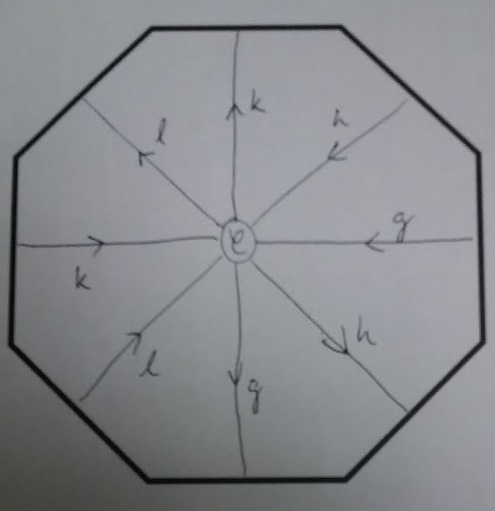
\includegraphics[width=0.5\textwidth]{basis.jpg}
\caption{Element of the spanning set $S$ for a genus 2 surface}
\label{fig:span}
\end{figure}

\begin{figure}
 \centering
 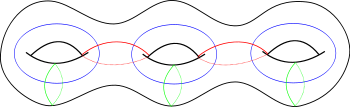
\includegraphics[width=.60\textwidth]{lickorish.png}
 \caption{Simple closed curves for the Dehn twists in the Lickorish generating set for the mapping class group of a genus $3$ closed surface (Image source: \url{https://en.wikipedia.org/wiki/Dehn_twist})}
\label{fig:lickorish}
\end{figure}



The mapping class group of $\Si$ is generated by the Lickorish generating set consisting of Dehn twists around $3g-1$ simple closed curves.   These can be divided into two types of twists: the ones around a single hole (the blue and green curves in Figure \ref{fig:lickorish}), and the ones connecting two holes (the red curves). The action of a Dehn twist around a simple closed curve corresponds to cutting the manifold along the curve, holding one piece in place and twisting the other piece by $2\pi$ radians in a clockwise direction, then gluing the two pieces back together.


To understand the action of each type of Dehn twist on the representation space $H$, we will consider the action on the spanning set $S$.  First, we claim that we can apply local moves to any element of $S$ to get a colored graph of the form shown in the first subfigure of Figure \ref{fig:tikzTwist1_1}, where the unshown part of the fundamental polygon looks the same as in the definition of $S$.  Indeed, to pass from an arbitrary element of $S$, to a colored graph of the form shown in the first subfigure of $\ref{fig:tikzTwist1_1}$, we first add coevalution-labeled vertices to each  edge intersecting the three shown sides of the fundamental polygon.  Then connect the new vertices using edges labeled by the trivial object (this corresponds to applying the second local move in Figure \ref{f:local_rels1} with  $k = 0$), contract the connections to get one new vertex, and tensor together the edges connecting the old vertex to the new vertex.

The action of the first type of Dehn twist on an arbitrary element of $S$ is shown in the first two subfigures of Figure \ref{fig:tikzTwist1_1}.  
After applying the Dehn twist, we have the simple colored graph shown in the second subfigure of Figure \ref{fig:tikzTwist1_1}.  We then apply local moves in the remaining subfigures.  For example, to go from the second subfigure to the third, we first apply the third local move of Figure \ref{f:local_rels1} to add a $\coev$-labeled vertex to the top left $g$-labeled edge.  We then apply the second local move (tensoring edges) with the number of parallel edges $k = 0$ to add an edge labeled by the trivial object between the new vertex and the old one. To go from the third to the fourth subfigure, we apply the edge contraction local move on the new edge.  Lastly, we get to the fifth subfigure by applying the tensoring edges local move again (strictly speaking, this is not a valid move since it does not take place on a disk, but one can easily add a $\coev$-labeled vertex to each of the two parallel edges, connect them, contract the connection, tensor together each of the two pairs of parallel edges, and contract one of the resulting edges to get the same result). By repeated application of Proposition $\ref{prop:omega}$, the resulting colored graph is equivalent to $\beta \Delta$, for some $\beta \in \mu_{|G|}$ and  $\Delta \in S$.    Thus, the first type of Dehn twist maps $S$ to $\mu_{|G|} S$.

An analogous proof works for the second type of Dehn twist shown in Figure \ref{fig:tikzTwist2_0}. Thus, the image of any such mapping class group representation is a quotient of the group of permutations of the finite set $\mu_{|G|} S$, hence finite.
\end{proof}

\begin{rmk} 
When $\omega = 1$ and $\Si$ is closed, this representation is a permutation representation.  
\end{rmk}

\begin{proof}
Under the assumption that the representation in \cite{fjfu} coincides with ours, this fact follows from Theorem 2.6 in \cite{fjfu}, but we can also prove it directly.  We first note that $G$ acts on $S$ by simultaneous conjugation of all edge labels by a single element $g \in G$.  If $s \in S$ and $g \in G$, then we can retrieve $s$ from $gs$ by separating two oppositely oriented, $g$-labeled edges from each edge in the embedded graph $gs$.  This results in a loop labeled by $g$, whose evaluation is $1$.  Thus $gs$ is equivalent to $s$.  Moreover, the cardinality $|S/G| = |\Hom(\pi_1(M), G)|/|G|$ is equal to the dimension of the untwisted Dijkgraaf-Witten representation space $H$ \cite{dijkgraaf1990}.  Hence, $S/G$ is a basis for $H$.  The mapping class group action on $S$ commutes with the $G$-action, so the mapping class group permutes $S/G$, i.e. $H$ is a permutation representation.
\end{proof}

\newcommand{\nc}{\newcommand}
\newcommand{\rnc}{\renewcommand}

%% Definitions

    % boundary of polygon
    % top left corner
     \nc{\lcx}{-0.5}
     \nc{\lcy}{0.866}
     \nc{\rcx}{-\lcx}
     \nc{\rcy}{\lcy}

     %TODO: Color edges
     \nc{\makeBdy}{
       \begin{scope}[very thick,decoration={
             markings,
             mark=at position 0.5 with {\arrow{>}}}
         ]  

         \draw (-1,0) -- (\lcx, \lcy); 
         \draw (\lcx, \lcy) -- (\rcx, \rcy); 
         \draw  (1, 0) -- (\rcx, \rcy);
       \end{scope}
     }

    %cut    
    % left endpoint of cut
    \nc{\lcutx}{-0.6}
    \nc{\lcuty}{0.6928}
    \nc{\lcut}{(\lcutx, \lcuty)}
    \nc{\rcutx}{-\lcutx}
    \nc{\rcuty}{\lcuty}
    \nc{\rcut}{(\rcutx, \rcuty)}

    %Main vertex
    \nc{\mvx}{0}
    \nc{\mvy}{0.2}
    \nc{\mv}{(\mvx, \mvy)}

    % outgoing edge
    \nc{\outEdge}{\draw[postaction={decorate}]  (0, 0) -- \mv node[pos=.5, right]{$hgh^{-1}$};}

    % middle of top edge of polygon
    \nc{\mtopx}{0}
    \nc{\mtopy}{0.866}
    \nc{\mtop}{(\mtopx, \mtopy)}

\begin{figure}
\centering

\begin{tabular}{|c|c|}

\hline

%Dehn twist 1.1
    \begin{tikzpicture}[scale=3]    

      % boundary of polygon
      \makeBdy


    \begin{scope}[very thick,decoration={
    markings,
    mark=at position 0.5 with {\arrow{>}}}
    ]  

      % cut for Dehn twist
      \draw[loosely dashed] \lcut -- \rcut;
      

      %graph edges

      \draw[postaction={decorate}]   \mv -- (0.75, 0.433) node[pos=.5,sloped,above]{$h$};
      \draw[postaction={decorate}]   \mv -- \mtop node[pos=.5,left]{$g$};
      \draw[postaction={decorate}]  (-0.75, 0.433) -- \mv node[pos=.5,sloped,above]{$h$};
      \outEdge

    \end{scope}
    \end{tikzpicture}

&

%1.2
    \begin{tikzpicture}[scale=3]
    
    %boundary of polygon
      \makeBdy

    %graph edges
    \begin{scope}[very thick,decoration={
    markings,
    mark=at position 0.5 with {\arrow{>}}}
    ] 


        \draw[postaction={decorate}]   \mv -- (0.75, 0.433) node[pos=.5,sloped,above]{$h$};
        % old g
        % \draw[postaction={decorate}]   \rb -- (0, 0.866) node[pos=.5,left]{$g$};
        \draw[postaction={decorate}]  (-0.75, 0.433) -- \mv node[pos=.5,sloped,above]{$h$};
        \outEdge

        % new g
        \draw[postaction={decorate}]  \mv -- \rcut
        node[pos=.5,sloped,above]{$g$};
        \draw[postaction={decorate}]  \lcut -- \mtop
        node[pos=.5,sloped,below]{$g$};

    \end{scope}
    \end{tikzpicture}

\\ \hline

%1.3
      \begin{tikzpicture}[scale=3]
    
    %boundary of polygon
      \makeBdy

    %graph edges
    \begin{scope}[very thick,decoration={
    markings,
    mark=at position 0.5 with {\arrow{>}}}
    ] 

        \draw[postaction={decorate}]   \mv -- (0.75, 0.433) node[pos=.5,sloped,above]{$h$};
        \draw[postaction={decorate}]  (-0.75, 0.433) -- \mv node[pos=.5,sloped,above]{$h$};

        \outEdge

        \draw[postaction={decorate}]  \mv -- \rcut
        node[pos=.5,sloped,above]{$g$};
        %\draw[postaction={decorate}]  \lcut -- \mtop
        \draw[postaction={decorate}]  \lcut --  ({(\lcutx + \mtopx)/2} , {(\lcuty + \mtopy)/2})
        node[pos=.5,sloped,below]{$g$};
        \draw[postaction={decorate}]  ({(\lcutx + \mtopx)/2} , {(\lcuty + \mtopy)/2}) -- \mtop
        node[pos=.5,sloped,below]{$g$};


        \draw  \mv --  ({(\lcutx + \mtopx)/2} , {(\lcuty + \mtopy)/2});

    \end{scope}
    \end{tikzpicture}

&

%1.4
    
    \begin{tikzpicture}[scale=3]

      %boundary of polygon
      \makeBdy


      
      \begin{scope}[very thick,decoration={
            markings,
            mark=at position 0.5 with {\arrow{>}}}
        ] 
      %graph edges

        \draw[postaction={decorate}]   \mv -- (0.75, 0.433) node[pos=.5,sloped,above]{$h$};
        \draw[postaction={decorate}]  (-0.75, 0.433) -- \mv node[pos=.5,sloped,above]{$h$};

        \outEdge

        \draw[postaction={decorate}]  \mv -- \rcut
        node[pos=.5,sloped,above]{$g$};
        %\draw[postaction={decorate}]  \lcut -- \mtop
        \draw[postaction={decorate}]  \lcut -- \mv
        node[pos=.5,sloped,above]{$g$};
        \draw[postaction={decorate}]  \mv -- \mtop
        node[pos=.5,right]{$g$};


    \end{scope}
    \end{tikzpicture}

\\ \hline

%Dehn twist 1.5

    
    \begin{tikzpicture}[scale=3]

    % boundary of polygon
     \makeBdy
    
    %graph edges
    \begin{scope}[very thick,decoration={
    markings,
    mark=at position 0.5 with {\arrow{>}}}
    ]  
        \draw[postaction={decorate}]   \mv -- (0.75, 0.433) node[pos=.5,sloped,above]{$hg$};
        \draw[postaction={decorate}]   \mv -- \mtop node[pos=.5,left]{$g$};
        \draw[postaction={decorate}]  (-0.75, 0.433) -- \mv node[pos=.5,sloped,above]{$hg$};
        \outEdge

    \end{scope}
    \end{tikzpicture}

&

\\ \hline
\end{tabular}

\caption{Using local moves to calculate the action of the first type of Dehn twist on an arbitrary element of the spanning set $S$. Read from left to right, then top to bottom.  Unlabeled interior edges are colored by the group identity element.  The Dehn twist is performed along the dashed simple closed curve.  The first two subfigures show the action of the Dehn twist.  The last three show the local moves relating the image of the Dehn twist to another element of $S$.}
\label{fig:tikzTwist1_1}
\end{figure}

%%%%%%%%%%%% Twist 2 %%%%%%%%%%%%%%%%


\nc{\makeBdyTwo}{
  \begin{scope}[very thick,decoration={
    markings,
    mark=at position 0.5 with {\arrow{>}}}
    ]  
    \path[draw]
    (1.0,          0.0) --       %0
    (0.92388,      0.382683)  -- %1
    (0.707107,     0.707107) --  %2
    (0.382683,     0.92388) --   %3
    (0,            1.0)   --     %4
    (-0.382683,    0.92388) --   %5
    (-0.707107 ,   0.707107)  -- %6
    ( -0.92388,    0.382683) --  %7
    ( -1.0     ,   0);           %8

  \end{scope}
}


\nc{\mvTwo}{ (-0.312076, 0.753418) }

\nc{\outEdgeTwo}{\draw[postaction={decorate}]  (0, 0) -- \mv node[pos=.3, right]{$[a,b][c,d]$};}

% 0.9 1 + 0.1 6
\nc{\cutOneX}{{0.8*(-0.92388) + 0.2*(-0.707107)}}
\nc{\cutOneY}{{0.8*(0.382683) + 0.2*(0.707107)}}
\nc{\cutOne}{(\cutOneX, \cutOneY)}

%0.9 3 + 0.1 4
\nc{\cutTwoX}{{0.8*(0.382683) + 0.2*(0)}}
\nc{\cutTwoY}{{0.8*(0.92388) + 0.2*(1.0)}}
\nc{\cutTwo}{(\cutTwoX, \cutTwoY)}

%0.9 2 + 0.1 1
\nc{\cutThreeX}{{0.8*(0.707107 ) + 0.2*(0.92388 )}}
\nc{\cutThreeY}{{0.8*(0.707107 ) + 0.2*(0.382638 )}}
\nc{\cutThree}{(\cutThreeX, \cutThreeY)}

%0.9 2 + 0.1 3
\nc{\cutFourX}{{0.2*( 0.382683) + 0.8*(0.707107)}}
\nc{\cutFourY}{{0.2*( 0.92388) + 0.8*(0.707107)}}
\nc{\cutFour}{(\cutFourX, \cutFourY)}

%0.1 0   0.9 1
\nc{\cutFiveX}{{0.2*( 1.0) + 0.8*(0.92388)}}
\nc{\cutFiveY}{{0.2*( 0.0) + 0.8*(0.382638)}}
\nc{\cutFive}{(\cutFiveX, \cutFiveY)}

%0.1 2   0.9 1
\nc{\cutSixX}{{0.2*( 0.707107) + 0.8*(0.92388)}}
\nc{\cutSixY}{{0.2*( 0.707107) + 0.8*(0.382683)}}
\nc{\cutSix}{(\cutSixX, \cutSixY)}

%0.1 3      0.9 4
\nc{\cutSevenX}{{0.2*( 0.382683) + 0.8*(0.0)}}
\nc{\cutSevenY}{{0.2*( 0.92388) + 0.8*(1.0)}}
\nc{\cutSeven}{(\cutSevenX, \cutSevenY)}

%0.1 5 0.9 4
\nc{\cutEightX}{{0.2*( -0.382683) + 0.8*(0.0)}}
\nc{\cutEightY}{{0.2*( 0.92388) + 0.8*(1.0)}}
\nc{\cutEight}{(\cutEightX, \cutEightY)}

\begin{figure}
\centering

\begin{tabular}{|c|c|}

\hline
%2.1    
    \begin{tikzpicture}[scale=3]

    % boundary of polygon
     \makeBdyTwo

     % cut for Dehn twist
     \draw[dotted] \cutOne -- \cutTwo;
     \draw[dotted] \cutThree -- \cutFour;
     \draw[dotted] \cutFive -- \cutSix;
     \draw[dotted] \cutSeven -- \cutEight;
         
    %graph edges
    \begin{scope}[very thick,decoration={
    markings,
    mark=at position 0.5 with {\arrow{>}}}
    ]  
       \draw[postaction={decorate}]  \mv -- (   0.96194 , 0.191342) node[pos=.5,sloped,above]{$a$};
       \draw[postaction={decorate}]  \mv -- ( 0.815493,  0.544895) node[pos=.5,sloped,above]{$b$};
       \draw[postaction={decorate}] (0.544895,  0.815493) -- \mv  node[pos=.5,sloped,above]{$a$};
       \draw[postaction={decorate}]   (0.191342,  0.96194) -- \mv  node[pos=.4,sloped,above]{$b$}; 
       \draw[postaction={decorate}]  \mv -- (-0.191342,  0.96194) node[pos=.4,sloped,above]{$c$}; 
       \draw[postaction={decorate}]  \mv -- (-0.544895,  0.815493) node[pos=.5,sloped,above]{$d$}; 
       \draw[postaction={decorate}] (-0.815493,  0.544895) -- \mv  node[pos=.5,sloped,above]{$c$};
       \draw[postaction={decorate}] (-0.96194,   0.191342) -- \mv  node[pos=.5,sloped,above]{$d$};

         \outEdgeTwo
    \end{scope}
    \end{tikzpicture}

&

%2.2
    
    \begin{tikzpicture}[scale=3]

    % boundary of polygon
     \makeBdyTwo

     % cut for Dehn twist
     \draw[dotted] \cutOne -- \cutTwo;
     \draw[dotted] \cutThree -- \cutFour;
     \draw[dotted] \cutFive -- \cutSix;
     \draw[dotted] \cutSeven -- \cutEight;
         
    %graph edges
    \begin{scope}[very thick,decoration={
    markings,
    mark=at position 0.5 with {\arrow{>}}}
    ]  
       \draw[postaction={decorate}]  \mv -- \mvTwo node[pos=.5,sloped,above]{\tiny $g := b^{-1}cdc^{-1}$};

       \draw[postaction={decorate}]  \mv -- (   0.96194 , 0.191342) node[pos=.5,sloped,above]{$a$};
       \draw[postaction={decorate}]  \mv -- ( 0.815493,  0.544895) node[pos=.5,sloped,above]{$b$};
       \draw[postaction={decorate}] (0.544895,  0.815493) -- \mv  node[pos=.5,sloped,above]{$a$};
       \draw[postaction={decorate}]   (0.191342,  0.96194) -- \mvTwo  node[pos=.5,sloped,above]{$b$}; 
       \draw[postaction={decorate}]  \mvTwo -- (-0.191342,  0.96194) node[pos=.5,sloped,above]{$c$}; 
       \draw[postaction={decorate}]  \mvTwo -- (-0.544895,  0.815493) node[pos=.5,sloped,above]{$d$}; 
       \draw[postaction={decorate}] (-0.815493,  0.544895) -- \mvTwo  node[pos=.5,sloped,above]{$c$};
       \draw[postaction={decorate}] (-0.96194,   0.191342) -- \mv  node[pos=.5,sloped,above]{$d$};

         \outEdgeTwo
    \end{scope}
    \end{tikzpicture}

\\ \hline

%2.3
    
    \begin{tikzpicture}[scale=3]

    % boundary of polygon
     \makeBdyTwo
         
    %graph edges
    \begin{scope}[very thick,decoration={
    markings,
    mark=at position 0.5 with {\arrow{>}}}
    ]  
       \draw[postaction={decorate}]  \mv -- \cutTwo node[pos=.5,sloped,above]{$g$};
       \draw[postaction={decorate}]  \cutOne -- \mvTwo node[pos=.5,sloped,below]{$g$};
       \draw[postaction={decorate}]  \cutThree -- \cutFour node[pos=.5,sloped,below]{$g$};
       \draw[postaction={decorate}]  \cutFive -- \cutSix node[pos=.5,sloped,below]{$g$};
       \draw[postaction={decorate}]  \cutSeven -- \cutEight node[pos=.5,sloped,red]{$g$};


       \draw[postaction={decorate}]  \mv -- (   0.96194 , 0.191342) node[pos=.5,sloped,above]{$a$};
       \draw[postaction={decorate}]  \mv -- ( 0.815493,  0.544895) node[pos=.5,sloped,above]{$b$};
       \draw[postaction={decorate}] (0.544895,  0.815493) -- \mv  node[pos=.5,sloped,above]{$a$};
       \draw[postaction={decorate}]   (0.191342,  0.96194) -- \mvTwo  node[pos=.5,sloped,below]{$b$}; 
       \draw[postaction={decorate}]  \mvTwo -- (-0.191342,  0.96194) node[pos=.5,sloped,above]{$c$}; 
       \draw[postaction={decorate}]  \mvTwo -- (-0.544895,  0.815493) node[pos=.5,sloped,above]{$d$}; 
       \draw[postaction={decorate}] (-0.815493,  0.544895) -- \mvTwo  node[pos=.5,sloped,above]{$c$};
       \draw[postaction={decorate}] (-0.96194,   0.191342) -- \mv  node[pos=.5,sloped,above]{$d$};

         \outEdgeTwo
    \end{scope}
    \end{tikzpicture}

&

%2.4
    
    \begin{tikzpicture}[scale=3]

    % boundary of polygon
     \makeBdyTwo
         
    %graph edges
    \begin{scope}[very thick,decoration={
    markings,
    mark=at position 0.5 with {\arrow{>}}}
    ]  
       \draw[postaction={decorate}]  \mv -- \cutTwo node[pos=.5,sloped,above]{$g$};
       \draw[postaction={decorate}]  \cutThree -- \mv node[pos=.3,sloped,above]{$g$};

       \draw[postaction={decorate}]  \mv -- ( 0.96194 , 0.191342) node[pos=.8,sloped,above]{$ag^{-1}$};
       \draw[postaction={decorate}]  \mv -- ( 0.815493,  0.544895) node[pos=.7,sloped,below]{$gb$};
       \draw[postaction={decorate}] (0.544895,  0.815493) -- \mv  node[pos=.2,sloped,above]{$ag^{-1}$};
       \draw[postaction={decorate}]   (0.191342,  0.96194) -- \mvTwo  node[pos=.5,sloped,below]{$gb$}; 
       \draw[postaction={decorate}]  \mvTwo -- (-0.191342,  0.96194) node[pos=.5,sloped,above]{$gc$}; 
       \draw[postaction={decorate}]  \mvTwo -- (-0.544895,  0.815493) node[pos=.5,sloped,above]{$d$}; 
       \draw[postaction={decorate}] (-0.815493,  0.544895) -- \mvTwo  node[pos=.5,sloped,below]{$gc$};
       \draw[postaction={decorate}] (-0.96194,   0.191342) -- \mv  node[pos=.5,sloped,above]{$d$};

         \outEdgeTwo
    \end{scope}
    \end{tikzpicture}

\\ \hline 

%2.5

    \begin{tikzpicture}[scale=3]

    % boundary of polygon
     \makeBdyTwo
         
    %graph edges
    \begin{scope}[very thick,decoration={
    markings,
    mark=at position 0.5 with {\arrow{>}}}
    ]  
       \draw[postaction={decorate}]  \mv -- \cutTwo node[pos=.8,sloped,red]{$g$};
       \draw[postaction={decorate}]  \cutThree -- \mv node[pos=.2,sloped,above]{$g$};

       \draw[postaction={decorate}]  \mv -- ( 0.96194 , 0.191342) node[pos=.8,sloped,above]{$ag^{-1}$};
       \draw[postaction={decorate}]  \mv -- ( 0.815493,  0.544895) node[pos=.7,sloped,below]{$gb$};
       \draw[postaction={decorate}] (0.544895,  0.815493) -- \mv  node[pos=.2,sloped,above]{$ag^{-1}$};
       \draw[postaction={decorate}]   (0.191342,  0.96194) -- \mv  node[pos=.2,sloped,above]{$gb$}; 
       \draw[postaction={decorate}]  \mv -- (-0.191342,  0.96194) node[pos=.8,sloped,below]{$gc$}; 
       \draw[postaction={decorate}]  \mv -- (-0.544895,  0.815493) node[pos=.7,sloped,above]{$d$}; 
       \draw[postaction={decorate}] (-0.815493,  0.544895) -- \mv  node[pos=.3,sloped,above]{$gc$};
       \draw[postaction={decorate}] (-0.96194,   0.191342) -- \mv  node[pos=.3,sloped,above]{$d$};

         \outEdgeTwo
    \end{scope}
    \end{tikzpicture}

&

%2.6

    \begin{tikzpicture}[scale=3]

    % boundary of polygon
     \makeBdyTwo
         
    %graph edges
    \begin{scope}[very thick,decoration={
    markings,
    mark=at position 0.5 with {\arrow{>}}}
    ]  

       \draw[postaction={decorate}]  \mv -- ( 0.96194 , 0.191342) node[pos=.8,sloped,above]{$ag^{-1}$};
       \draw[postaction={decorate}]  \mv -- ( 0.815493,  0.544895) node[pos=.8,sloped,above]{$gbg^{-1}$};
       \draw[postaction={decorate}] (0.544895,  0.815493) -- \mv  node[pos=.2,sloped,above]{$ag^{-1}$};
       \draw[postaction={decorate}]   (0.191342,  0.96194) -- \mv  node[pos=.2,sloped,above]{$gbg^{-1}$}; 
       \draw[postaction={decorate}]  \mv -- (-0.191342,  0.96194) node[pos=.8,sloped,below]{$gc$}; 
       \draw[postaction={decorate}]  \mv -- (-0.544895,  0.815493) node[pos=.7,sloped,above]{$d$}; 
       \draw[postaction={decorate}] (-0.815493,  0.544895) -- \mv  node[pos=.3,sloped,above]{$gc$};
       \draw[postaction={decorate}] (-0.96194,   0.191342) -- \mv  node[pos=.3,sloped,above]{$d$};

         \outEdgeTwo
    \end{scope}
    \end{tikzpicture}

\\ \hline
\end{tabular}

\caption{Using local moves to calculate the action of the second type of Dehn twist on an arbitrary element of the spanning set $S$. Read from left to right, then top to bottom.   The Dehn twist is performed along the dashed simple closed curve.  The first two subfigures show application of local moves prior to the Dehn twist action. The third shows the action of the twist.  The last three show the local moves relating the image of the Dehn twist to another element of $S$.}
\label{fig:tikzTwist2_0}
\end{figure}


\subsection{Boundary Case}

When $\Si$ has boundary, we denote by $\MCG(\Si)$ the group of isotopy classes of homeomorphisms fixing the boundary of $\Si$ setwise. Given any labelling of the boundary  by objects in the Drinfeld center, $l : \pi_0(\partial M) \to \Obj(Z(\vgo))$, we get a mapping class group representation. The representation space is $\Hs(\Si, \VV)$ with boundary condition $\VV = F \circ l$, where $F$ is the forgetful functor $F: Z(\vgo) \to \vgo$.  The same local relations are valid in this representation space \cite{kirillovStringNets}.

By a similar argument as in the proof of the Theorem $\ref{thm:closed}$, any such representation space has a finite spanning set $S$ consisting of all simple colored graphs with a single vertex, loops for each of the usual generators of the fundamental group of $\Si$, and a leg from the vertex to each of the boundary components.  

Let $N$ denote the closed surface obtained by filling in all the boundary components of $\Si$ with disks. The mapping class group $\MCG(\Si)$ is generated by the same Dehn twists as $\MCG(N)$, as well as braids interchanging boundary components and mapping classes corresponding to dragging a boundary component along a representative of a standard generator of $\pi_1(N)$ \cite{birman}.  As in the proof of Theorem \ref{thm:closed}, applying any of these generators of $\MCG(\Si)$ to a colored graph in $S$ yields an element in $\mu_{|G|}S$ (see Figures \ref{fig:braid1} and \ref{fig:drag1}).  Since the braid group is also generated by such braids, we have the following theorem.


\nc{\rightX}{0.5}  % left marked point x value
\nc{\leftX}{-\rightX} % right marked point x value
\nc{\pY}{0.5}  % y value for marked points
\nc{\loopR}{0.3}
\renewcommand{\mv}{(0, -0.2)}

\nc{\makeBase}{
      % left loop
       \draw[very thick]  \mv -- ({\leftX - \loopR}, \pY);
       \draw[very thick]   ({\leftX + \loopR}, \pY) -- \mv;
       
       \begin{scope}[very thick,decoration={
             markings,
             mark=at position 0.5 with {\arrow{>}}}
         ]  

         % left leg
         \draw[postaction={decorate}]  \mv -- (\leftX, \pY) node[pos=.5,above]{$l$};

       \end{scope}

       % new right loop and leg
       \draw[very thick]  \mv -- ({\leftX - 4*\loopR}, \pY);
       \draw[very thick]   ({\leftX - 2*\loopR}, \pY) -- \mv;
 
       % right leg
       \draw[very thick]  \mv -- ({\leftX - 3*\loopR}, \pY);       

}


\nc{\makeBaseTwo}{
    % left loop

       \draw[very thick]   ({\leftX + \loopR}, \pY) -- \mv;
       
       \begin{scope}[very thick,decoration={
             markings,
             mark=at position 0.5 with {\arrow{>}}}
         ]  

         % left leg
         \draw[postaction={decorate}]  \mv -- (\leftX, \pY) node[pos=.5,above]{$l$};

       \end{scope}
  
       \draw[very thick]   ({\leftX - 2*\loopR}, \pY) -- \mv;
}


%bottom right of right loop
\nc{\bRight}{
        \begin{scope}[very thick,decoration={
           markings,
           mark=at position 0.5 with {\arrow{>}}}
       ]  
       \draw[postaction={decorate}]   plot[domain=360:180] ({\loopR*cos(\x) + \leftX + 3*\loopR}, {\loopR*sin(\x) + \pY});
       \node[below] at  ({\loopR*cos(270) + \leftX + 3*\loopR}, {\loopR*sin(270) + \pY}) {$g$};
     \end{scope}
   }

\nc{\makeBraid}{

     \makeBase

     \begin{scope}[very thick,decoration={
           markings,
           mark=at position 0.5 with {\arrow{>}}}
       ]  

       % left loop
       \draw[postaction={decorate}]   plot[domain=180:0]  
              ({\loopR*cos(\x) + \leftX}, {\loopR*sin(\x) + \pY});
       \node[above] at  ({\loopR*cos(90) + \leftX}, {\loopR*sin(90) + \pY}) {$k$};

       % right loop
       \draw[postaction={decorate}]     plot[domain=0:180] ({2*\loopR*cos(\x) + \leftX}, {2*\loopR*sin(\x) + \pY});
       \node[above] at  ({2*\loopR*cos(90) + \leftX}, {2*\loopR*sin(90) + \pY}) {$g$};
       \draw[postaction={decorate}]      plot[domain=180:0] ({4*\loopR*cos(\x) + \leftX}, {4*\loopR*sin(\x) + \pY});
       \node[above] at  ({4*\loopR*cos(90) + \leftX}, {4*\loopR*sin(90) + \pY}) {$g$};

       %\right leg
       \draw[postaction={decorate}]      plot[domain=180:0] ({3*\loopR*cos(\x) + \leftX}, {3*\loopR*sin(\x) + \pY});
       \node[above] at  ({3*\loopR*cos(90) + \leftX}, {3*\loopR*sin(90) + \pY}) {$h$};

     \end{scope}

     \bRight
       
}


\nc{\makeBraidOne}{

     \makeBase

     \begin{scope}[very thick,decoration={
           markings,
           mark=at position 0.25 with {\arrow{>}},
          mark=at position 0.75 with {\arrow{>}}}
       ]  

       % left loop
       \draw[postaction={decorate}]   plot[domain=180:0]  
              ({\loopR*cos(\x) + \leftX}, {\loopR*sin(\x) + \pY});
       \node[above] at  ({\loopR*cos(45) + \leftX}, {\loopR*sin(45) + \pY}) {$k$};
       \node[above] at  ({\loopR*cos(135) + \leftX}, {\loopR*sin(135) + \pY}) {$k$};

       % right loop
       \draw[postaction={decorate}]     plot[domain=0:180] ({2*\loopR*cos(\x) + \leftX}, {2*\loopR*sin(\x) + \pY});
       \node[above] at  ({2*\loopR*cos(45) + \leftX}, {2*\loopR*sin(45) + \pY}) {$g$};
       \node[above] at  ({2*\loopR*cos(135) + \leftX}, {2*\loopR*sin(135) + \pY}) {$g$};
       \draw[postaction={decorate}]      plot[domain=180:0] ({4*\loopR*cos(\x) + \leftX}, {4*\loopR*sin(\x) + \pY});
       \node[above] at  ({4*\loopR*cos(45) + \leftX}, {4*\loopR*sin(45) + \pY}) {$g$};
       \node[above] at  ({4*\loopR*cos(135) + \leftX}, {4*\loopR*sin(135) + \pY}) {$g$};

       %\right leg
       \draw[postaction={decorate}]      plot[domain=180:0] ({3*\loopR*cos(\x) + \leftX}, {3*\loopR*sin(\x) + \pY});
       \node[above] at  ({3*\loopR*cos(45) + \leftX}, {3*\loopR*sin(45) + \pY}) {$h$};
       \node[above] at  ({3*\loopR*cos(135) + \leftX}, {3*\loopR*sin(135) + \pY}) {$h$};

     \end{scope}

     \bRight       
}


\nc{\makeBraidTwo}{

     \makeBase


     \begin{scope}[very thick,decoration={
           markings,
           mark=at position 0.1 with {\arrow{>}},
          mark=at position 0.9 with {\arrow{>}}}
       ]  
       % \right leg
       \draw[postaction={decorate}]      plot[domain=180:0] ({3*\loopR*cos(\x) + \leftX}, {3*\loopR*sin(\x) + \pY});
       \node[right] at  ({3*\loopR*cos(18) + \leftX}, {3*\loopR*sin(18) + \pY}) {$h$};
       \node[left] at  ({3*\loopR*cos(162) + \leftX}, {3*\loopR*sin(162) + \pY}) {$h$};

       % left loop
       \draw[postaction={decorate}]      plot[domain=180:0] ({\loopR*cos(\x) + \leftX}, {3*\loopR*sin(\x) + \pY});
       \node[left] at  ({\loopR*cos(18) + \leftX}, {3*\loopR*sin(18) + \pY}) {$k$};
       \node[left] at  ({\loopR*cos(162) + \leftX}, {3*\loopR*sin(162) + \pY}) {$k$};
     \end{scope}

       % right loop
     \begin{scope}[very thick,decoration={
           markings,
           mark=at position 0.9 with {\arrow{>}}}]
       \draw[postaction={decorate}]         plot[domain=0:180] ({2*\loopR*cos(\x) + \leftX}, {3*\loopR*sin(\x) + \pY});
       \node[left] at  ({2*\loopR*cos(162) + \leftX}, {3*\loopR*sin(162) + \pY}) {$g$};
     \end{scope}
     \begin{scope}[very thick,decoration={
           markings,
           mark=at position 0.1 with {\arrow{>}}}]
     \draw[postaction={decorate}]       plot[domain=180:0] ({4*\loopR*cos(\x) + \leftX}, {3*\loopR*sin(\x) + \pY});
       \node[left] at  ({4*\loopR*cos(162) + \leftX}, {3*\loopR*sin(162) + \pY}) {$g$};
     \end{scope}
         
       \bRight
}

\nc{\makeBraidThree}{

  \makeBaseTwo

     \begin{scope}[very thick,decoration={
           markings,
          mark=at position 0.8 with {\arrow{>}}}
       ]  
       % \right leg
       \draw[postaction={decorate}]      plot[domain=90:0] ({3*\loopR*cos(\x) + \leftX}, {3*\loopR*sin(\x) + \pY});
       \node[right] at  ({3*\loopR*cos(18) + \leftX}, {3*\loopR*sin(18) + \pY}) {$h$};

       % left loop
       \draw[postaction={decorate}]      plot[domain=90:0] ({\loopR*cos(\x) + \leftX}, {3*\loopR*sin(\x) + \pY});
       \node[left] at  ({\loopR*cos(18) + \leftX}, {3*\loopR*sin(18) + \pY}) {$k$};
     \end{scope}

       % right loop
     \begin{scope}[very thick,decoration={
           markings,
           mark=at position 0.1 with {\arrow{>}}}]
       \draw[postaction={decorate}]         plot[domain=180:0] ({2*\loopR*cos(\x) + \leftX}, {3*\loopR*sin(\x) + \pY});
       \node[left] at  ({2*\loopR*cos(162) + \leftX}, {3*\loopR*sin(162) + \pY}) {$kg^{-1}hg$};
     \end{scope}

     \draw[very thick]       plot[domain=90:0] ({4*\loopR*cos(\x) + \leftX}, {3*\loopR*sin(\x) + \pY});
         
       \bRight
}


\begin{figure}
\centering

\begin{tabular}{|c|c|}

  \hline
  
  %Braid 1
    \begin{tikzpicture}[scale=2.5]

         
    %graph edges
    \begin{scope}[very thick,decoration={
    markings,
    mark=at position 0.5 with {\arrow{>}}}
    ]  


       % left loop
       \draw  \mv -- ({\leftX - \loopR}, \pY);
       \draw[postaction={decorate}]    plot[domain=180:0] ({\loopR*cos(\x) + \leftX}, {\loopR*sin(\x) + \pY});
       \node[above] at ({\loopR*cos(90) + \leftX}, {\loopR*sin(90) + \pY}) {$g$};
       \draw   ({\leftX + \loopR}, \pY) -- \mv;
       
       % left leg
       \draw[postaction={decorate}]  \mv -- (\leftX, \pY) node[pos=.5,above]{$h$};

       % right loop
       \draw  \mv -- ({\rightX - \loopR}, \pY);
       \draw[postaction={decorate}] plot[domain=180:0] ({\loopR*cos(\x) + \rightX}, {\loopR*sin(\x) + \pY});
       \node[above] at ({\loopR*cos(90) + \rightX}, {\loopR*sin(90) + \pY}) {$k$};
       \draw   ({\rightX + \loopR}, \pY) -- \mv;
 
       % right leg
       \draw[postaction={decorate}]  \mv -- (\rightX, \pY) node[pos=.5, above]{$l$};       
  
    \end{scope}
    \end{tikzpicture}

&

  %Braid 2
    \begin{tikzpicture}[scale=2.5]

         
    %graph edges
    \begin{scope}[very thick,decoration={
    markings,
    mark=at position 0.5 with {\arrow{>}}}
    ]  

    \makeBraid
  
    \end{scope}
    \end{tikzpicture}

\\ \hline

  %Braid 3
    \begin{tikzpicture}[scale=2.5]

      \makeBraidOne
         
    %graph edges
    \begin{scope}[very thick,decoration={
    markings,
    mark=at position 0.5 with {\arrow{>}}}
    ]  

       % connecting edge
       \draw ({\leftX}, {\pY + \loopR}) -- ({\leftX}, {\pY + 4*\loopR});
  
    \end{scope}
    \end{tikzpicture}

&

  %Braid 4
    \begin{tikzpicture}[scale=2.5]

      \makeBraidTwo     
         
    \end{tikzpicture}

\\ \hline

    %Braid 5
    \begin{tikzpicture}[scale=2.5]

      \makeBraidThree
         
    \end{tikzpicture}

&

  %Braid 6
    \begin{tikzpicture}[scale=2.5]

         
    %graph edges
    \begin{scope}[very thick,decoration={
    markings,
    mark=at position 0.5 with {\arrow{>}}}
    ]  


       % left loop
       \draw  \mv -- ({\leftX - \loopR}, \pY);
       \draw[postaction={decorate}]    plot[domain=180:0] ({\loopR*cos(\x) + \leftX}, {\loopR*sin(\x) + \pY});
       \node[above] at ({\loopR*cos(90) + \leftX}, {\loopR*sin(90) + \pY}) {$kg^{-1}hg$};
       \draw   ({\leftX + \loopR}, \pY) -- \mv;
       
       % left leg
       \draw[postaction={decorate}]  \mv -- (\leftX, \pY) node[pos=.5,above]{$l$};

       % right loop
       \draw  \mv -- ({\rightX - \loopR}, \pY);
       \draw[postaction={decorate}] plot[domain=180:0] ({\loopR*cos(\x) + \rightX}, {\loopR*sin(\x) + \pY});
       \node[above] at ({\loopR*cos(90) + \rightX}, {\loopR*sin(90) + \pY}) {$g$};
       \draw   ({\rightX + \loopR}, \pY) -- \mv;
 
       % right leg
       \draw[postaction={decorate}]  \mv -- (\rightX, \pY) node[pos=.5, above]{$h$};       
  
    \end{scope}
    \end{tikzpicture}

\\ \hline
\end{tabular}

\caption{Using local moves to calculate the action of a braid generator on an arbitrary element of the spanning set $S$. Read from left to right, then top to bottom.   Unlabeled interior edges are colored by the group identity element. The first two subfigures show application of the braid generator, which interchanges the univalent vertices. The last four show the local moves relating the image to another element of $S$.}
\label{fig:braid1}
\end{figure}


%%%%%%%%%%%%%%%%%% Dragging along \pi_1 generator %%%%%%%%%

\rnc{\mv}{(0,0)}
\nc{\uv}{(0, 0.7)}
\nc{\rvx}{0.3}
\nc{\rvy}{\lcuty}
\nc{\rv}{(\rvx, \rvy)}
\nc{\lv}{(-\rvx, \lcuty)}

\nc{\cutRatio}{0.5}
\rnc{\lcutx}{{\cutRatio*(-0.5) + (1-\cutRatio)*(-1)}}
\rnc{\lcuty}{{\cutRatio*(0.866)}}
\rnc{\lcut}{(\lcutx, \lcuty)}
\rnc{\rcutx}{{\cutRatio*(0.5) + (1-\cutRatio)*(1)}}
\rnc{\rcut}{(\rcutx, \lcuty)}
\nc{\boundaryComponentx}{0}
\nc{\boundaryComponenty}{\lcuty}
\nc{\boundaryComponent}{(\boundaryComponentx, \boundaryComponenty)}

\nc{\connectorEnd}{({0.5*(-0.85)}, {0.5*0.2598 + 0.5*0.433})}

\nc{\edgeRatio}{0.9}
\nc{\lex}{{\edgeRatio*(-1) + (1-\edgeRatio)*(\lcx)}}
\nc{\ley}{{(1-\edgeRatio)*(\lcy)}}
\nc{\lev}{(\lex, \ley)}
%\nc{\rex}{{(-1)*(\lex)}}
\nc{\rex}{{\edgeRatio*(1) + (1-\edgeRatio)*(\rcx)}}
\nc{\rev}{(\rex, \ley)}

\nc{\eOneRatio}{0.8}
\nc{\leOnex}{{\eOneRatio*(-1) + (1-\eOneRatio)*(\lcx)}}
\nc{\leOney}{{(1-\eOneRatio)*(\lcy)}}
\nc{\leOnev}{(\leOnex, \leOney)}
\nc{\reOnex}{{\eOneRatio*(1) + (1-\eOneRatio)*(\rcx)}}
\nc{\reOnev}{(\reOnex, \leOney)}

\nc{\eTwoRatio}{0.7}
\nc{\leTwox}{{\eTwoRatio*(-1) + (1-\eTwoRatio)*(\lcx)}}
\nc{\leTwoy}{{(1-\eTwoRatio)*(\lcy)}}
\nc{\leTwov}{(\leTwox, \leTwoy)}
\nc{\reTwox}{{\eTwoRatio*(1) + (1-\eTwoRatio)*(\rcx)}}
\nc{\reTwov}{(\reTwox, \leTwoy)}

\nc{\eThreeRatio}{0.6}
\nc{\leThreex}{{\eThreeRatio*(-1) + (1-\eThreeRatio)*(\lcx)}}
\nc{\leThreey}{{(1-\eThreeRatio)*(\lcy)}}
\nc{\leThreev}{(\leThreex, \leThreey)}
\nc{\reThreex}{{\eThreeRatio*(1) + (1-\eThreeRatio)*(\rcx)}}
\nc{\reThreev}{(\reThreex, \leThreey)}

\nc{\eFourRatio}{0.4}
\nc{\leFourx}{{\eFourRatio*(-1) + (1-\eFourRatio)*(\lcx)}}
\nc{\leFoury}{{(1-\eFourRatio)*(\lcy)}}
\nc{\leFourv}{(\leFourx, \leFoury)}
\nc{\reFourx}{{\eFourRatio*(1) + (1-\eFourRatio)*(\rcx)}}
\nc{\reFourv}{(\reFourx, \leFoury)}

\nc{\eFiveRatio}{0.2}
\nc{\leFivex}{{\eFiveRatio*(-1) + (1-\eFiveRatio)*(\lcx)}}
\nc{\leFivey}{{(1-\eFiveRatio)*(\lcy)}}
\nc{\leFivev}{(\leFivex, \leFivey)}
\nc{\reFivex}{{\eFiveRatio*(1) + (1-\eFiveRatio)*(\rcx)}}
\nc{\reFivev}{(\reFivex, \leFivey)}


\nc{\dby}{-0.2} %diagram bottom

\begin{figure}
\centering

\begin{tabular}{|c|c|}

  \hline
  
  % Drag 1
    \begin{tikzpicture}[scale=3]    

      % boundary of polygon
      \makeBdy


    \begin{scope}[very thick,decoration={
    markings,
    mark=at position 0.5 with {\arrow{>}}}
    ]  

      % cut for Dehn twist
      \draw[loosely dashed] \lcut -- \rcut;
      

      %graph edges
      \draw[postaction={decorate}]   (0, \dby) -- \mv node[pos=.5,right]{$p:=hglkl^{-1}h^{-1}$};
      \draw[postaction={decorate}]   \mv -- \rev node[pos=.5,sloped,above]{$h$};
      \draw[postaction={decorate}]   \mv -- \rv node[pos=.5,right]{$gl$};
      \draw[postaction={decorate}]   \mv -- \boundaryComponent node[pos=.5,left]{$k$};
      \draw[postaction={decorate}]   \lv -- \mv node[pos=.5,left]{$l$};
      \draw[postaction={decorate}]   \lev -- \mv node[pos=.5,sloped,below]{$h$};

      \draw[postaction={decorate}]   \rv -- \uv;
      \draw[postaction={decorate}]   \uv -- \mtop node[pos=.5,right]{$g$};
      \draw[postaction={decorate}]   \uv -- \lv;


    \end{scope}
    \end{tikzpicture}


&


  % Drag 2
    \begin{tikzpicture}[scale=3]    

      % boundary of polygon
      \makeBdy


    \begin{scope}[very thick,decoration={
    markings,
    mark=at position 0.5 with {\arrow{>}}}
    ]  


      %graph edges
      \draw[postaction={decorate}]   (0, \dby) -- \mv node[pos=.5,right]{$p$};
      \draw[postaction={decorate}]   \mv -- \rev node[pos=.5,sloped,below]{$h$};

      \draw[postaction={decorate}]   \mv -- \reOnev node[pos=.8,sloped,red]{$gl$};
      \draw[postaction={decorate}]   \leOnev -- \rv node[pos=.5,sloped,below]{$gl$};
      \draw[postaction={decorate}]   \rv -- \leFivev node[pos=.5,sloped,above]{$gl$};
      \draw[postaction={decorate}]   \reFivev -- \uv node[pos=.5,sloped,above]{$gl$};

      \draw[postaction={decorate}]   \mv -- \reTwov node[pos=.6,sloped,red]{$k$};
      \draw[postaction={decorate}]   \leTwov -- \boundaryComponent node[pos=.5,sloped,red]{$k$};

      \draw[postaction={decorate}]   \reThreev -- \mv node[pos=.5,sloped,above]{$l$};
      \draw[postaction={decorate}]   \lv -- \leThreev;
      \draw[postaction={decorate}]   \leFourv -- \lv node[pos=.5,sloped,above]{$l$};
      \draw[postaction={decorate}]   \uv -- \reFourv node[pos=.5,sloped,below]{$l$};

      \draw[postaction={decorate}]   \lev -- \mv node[pos=.5,sloped,below]{$h$};

      \draw[postaction={decorate}]   \uv -- \mtop node[pos=.5,right]{$g$};


    \end{scope}
    \end{tikzpicture}

\\ \hline


  % Drag 3
    \begin{tikzpicture}[scale=3]    

      % boundary of polygon
      \makeBdy

    \begin{scope}[very thick,decoration={
    markings,
    mark=at position 0.5 with {\arrow{>}}}
    ]  


      %graph edges
      \draw[postaction={decorate}]   (0, \dby) -- \mv node[pos=.5,right]{$p$};
      \draw[postaction={decorate}]   \mv -- \rev node[pos=.5,sloped,below]{$h$};

      \draw[postaction={decorate}]   \mv -- \reOnev node[pos=.8,sloped,red]{$gl$};
      \draw[postaction={decorate}]   \leOnev --  (-0.35, 0.3031) node[pos=.5,sloped,below]{$gl$};
      \draw[postaction={decorate}]   (-0.35, 0.3031) -- \rv node[pos=.5,sloped,below]{$gl$};

      \draw[postaction={decorate}]   \rv -- \leFivev node[pos=.5,sloped,above]{$gl$};
      \draw[postaction={decorate}]   \reFivev -- \uv node[pos=.5,sloped,above]{$gl$};

      \draw[postaction={decorate}]   \mv -- \reTwov node[pos=.6,sloped,red]{$k$};
      \draw[postaction={decorate}]   \leTwov -- \connectorEnd node[pos=.5,sloped,red]{$k$};
      \draw[postaction={decorate}]   \connectorEnd -- \boundaryComponent node[pos=.5,sloped,red]{$k$};


      \draw[postaction={decorate}]   \reThreev -- \mv node[pos=.5,sloped,above]{$l$};
      \draw[postaction={decorate}]   \lv -- \leThreev;
      \draw[postaction={decorate}]   \leFourv -- \lv node[pos=.5,sloped,above]{$l$};
      \draw[postaction={decorate}]   \uv -- \reFourv node[pos=.5,sloped,below]{$l$};

      \draw[postaction={decorate}]   \lev -- \mv node[pos=.5,sloped,below]{$h$};

      \draw[postaction={decorate}]   \uv -- \mtop node[pos=.5,right]{$g$};

      \draw \lcut -- \lv;
      \draw \rv -- \rcut;
      \draw \mv -- \connectorEnd;
     
    \end{scope}
    \end{tikzpicture}

&


  % Drag 4
    \begin{tikzpicture}[scale=3]    

      % boundary of polygon
      \makeBdy

    \begin{scope}[very thick,decoration={
    markings,
    mark=at position 0.5 with {\arrow{>}}}
    ]  


      %graph edges
      \draw[postaction={decorate}]   (0, \dby) -- \mv node[pos=.5,right]{$p$};
      \draw[postaction={decorate}]   \mv -- \rev node[pos=.5,sloped,below]{$h$};

      \draw[postaction={decorate}]   \mv -- \reOnev node[pos=.5,sloped,above]{$glk$};
      \draw[postaction={decorate}]   \leOnev --  (-0.35, 0.3031) node[pos=.5,sloped,above]{$glk$};
      \draw[postaction={decorate}]   (-0.35, 0.3031) -- \rv node[pos=.5,sloped,below]{$gl$};

      \draw[postaction={decorate}]   \rv -- \leFivev node[pos=.5,sloped,above]{$gl$};
      \draw[postaction={decorate}]   \reFivev -- \uv node[pos=.5,sloped,above]{$gl$};

      \draw[postaction={decorate}]    (-0.35, 0.3031)  -- \boundaryComponent node[pos=.5,sloped,above]{$k$};


      \draw[postaction={decorate}]   \rv -- \mv node[pos=.5,right]{$l$};
      \draw[postaction={decorate}]   \uv -- \rv node[pos=.5,right]{$l$};

      \draw[postaction={decorate}]   \lev -- \mv node[pos=.5,sloped,below]{$h$};

      \draw[postaction={decorate}]   \uv -- \mtop node[pos=.5,right]{$g$};


      \draw \mv --  (-0.35, 0.3031);
     
    \end{scope}
    \end{tikzpicture}


\\ \hline

  % Drag 5

 \begin{tikzpicture}[scale=3]    

      % boundary of polygon
      \makeBdy

    \begin{scope}[very thick,decoration={
    markings,
    mark=at position 0.5 with {\arrow{>}}}
    ]  


      %graph edges
      \draw[postaction={decorate}]   (0, \dby) -- \mv node[pos=.5,right]{$p$};
      \draw[postaction={decorate}]   \mv -- \rev node[pos=.5,sloped,below]{$hglk$};

      \draw[postaction={decorate}]   \rv -- \leFivev node[pos=.5,sloped,above]{$gl$};
      \draw[postaction={decorate}]   \reFivev -- \uv node[pos=.5,sloped,above]{$gl$};

      \draw[postaction={decorate}]    \mv  -- \boundaryComponent node[pos=.5,left]{$k$};


      \draw[postaction={decorate}]   \mv -- \rv node[pos=.5,right]{$l^{-1}gl$};
      \draw[postaction={decorate}]   \uv -- \rv node[pos=.5,right]{$l$};

      \draw[postaction={decorate}]   \lev -- \mv node[pos=.5,sloped,below]{$hglk$};

      \draw[postaction={decorate}]   \uv -- \mtop node[pos=.5,right]{$g$};
     
    \end{scope}
    \end{tikzpicture}

&


  % Drag 6

 \begin{tikzpicture}[scale=3]    

      % boundary of polygon
      \makeBdy

    \begin{scope}[very thick,decoration={
    markings,
    mark=at position 0.5 with {\arrow{>}}}
    ]  


      %graph edges
      \draw[postaction={decorate}]   (0, \dby) -- \mv node[pos=.5,right]{$p$};
      \draw[postaction={decorate}]   \mv -- \rev node[pos=.5,sloped,below]{$hglk$};

      \draw[postaction={decorate}]   \uv -- \leFivev node[pos=.5,sloped,below]{$gl$};
      \draw[postaction={decorate}]   \reFivev -- \uv node[pos=.5,sloped,below]{$gl$};

      \draw[postaction={decorate}]    \mv  -- \boundaryComponent node[pos=.5,left]{$k$};


      \draw[postaction={decorate}]   \mv -- \rv node[pos=.5,right]{$l^{-1}gl$};
      \draw[postaction={decorate}]   \rv -- \uv;

      \draw[postaction={decorate}]   \lev -- \mv node[pos=.5,sloped,below]{$hglk$};

      \draw[postaction={decorate}]   \uv -- \mtop node[pos=.5,right]{$g$};

     
    \end{scope}
    \end{tikzpicture}

\\ \hline

  % Drag 7

   \begin{tikzpicture}[scale=3]    

      % boundary of polygon
      \makeBdy

    \begin{scope}[very thick,decoration={
    markings,
    mark=at position 0.5 with {\arrow{>}}}
    ]  


      %graph edges
      \draw[postaction={decorate}]   (0, \dby) -- \mv node[pos=.5,right]{$p$};
      \draw[postaction={decorate}]   \mv -- \rev node[pos=.5,sloped,below]{$hglk$};

      \draw[postaction={decorate}]   \rev -- \uv node[pos=.5,sloped,above]{$gl$};
      \draw[postaction={decorate}]   \uv -- \lev node[pos=.5,sloped,above]{$gl$};

      \draw[postaction={decorate}]    \mv  -- \boundaryComponent node[pos=.5,left]{$k$};

      \draw[postaction={decorate}]   \mv -- \rv node[pos=.5,right]{$l^{-1}gl$};
      \draw[postaction={decorate}]   \rv -- \uv;

      \draw[postaction={decorate}]   \lev -- \mv node[pos=.5,sloped,below]{$hglk$};
      
      \draw[postaction={decorate}]   \uv -- \mtop node[pos=.5,right]{$g$};;

     
    \end{scope}
    \end{tikzpicture}

&

 % Drag 8
 \begin{tikzpicture}[scale=3]    

      % boundary of polygon
      \makeBdy

    \begin{scope}[very thick,decoration={
    markings,
    mark=at position 0.5 with {\arrow{>}}}
    ]  


      %graph edges
      \draw[postaction={decorate}]   (0, \dby) -- \mv node[pos=.5,right]{$p$};
      \draw[postaction={decorate}]   \mv -- \rev node[pos=.5,sloped,below]{$hglk$};

      \draw[postaction={decorate}]   \uv -- \leTwov  node[pos=.5,sloped,below]{$gl$};
      \draw[postaction={decorate}]   \reTwov -- \mv  node[pos=.5,sloped,above]{$gl$};

      \draw[postaction={decorate}]    \mv  -- \boundaryComponent node[pos=.5,left]{$k$};


      \draw[postaction={decorate}]   \mv -- \rv;
      \draw[postaction={decorate}]   \rv -- \uv node[pos=.5,right]{$g^2l$};

      \draw[postaction={decorate}]   \lev -- \mv node[pos=.5,sloped,below]{$hglk$};
      
      \draw[postaction={decorate}]   \uv -- \mtop node[pos=.5,right]{$g$};

     
    \end{scope}
    \end{tikzpicture}



\\ \hline


 % Drag 9
 \begin{tikzpicture}[scale=3]    

      % boundary of polygon
      \makeBdy

    \begin{scope}[very thick,decoration={
    markings,
    mark=at position 0.5 with {\arrow{>}}}
    ]  


      %graph edges
      \draw[postaction={decorate}]   (0, \dby) -- \mv node[pos=.5,right]{$p$};
      \draw[postaction={decorate}]   \mv -- \rev node[pos=.5,sloped,below]{$hglk$};

      \draw[postaction={decorate}]   \uv -- \leTwov node[pos=.5,sloped,below]{$gl$};
      \draw[postaction={decorate}]   \reTwov -- \mv node[pos=.5,sloped,above]{$gl$};
      \draw \leTwov -- \mv;

      \draw[postaction={decorate}]    \mv  -- \boundaryComponent node[pos=.5,left]{$k$};


      \draw[postaction={decorate}]   \mv -- \rv;
      \draw[postaction={decorate}]   \rv -- \uv node[pos=.5,right]{$g^2l$};

      \draw[postaction={decorate}]   \lev -- \mv node[pos=.5,sloped,below]{$hglk$};
      
      \draw[postaction={decorate}]   \uv -- \mtop node[pos=.5,right]{$g$};


     
    \end{scope}
    \end{tikzpicture}

&

% Drag 10

 \begin{tikzpicture}[scale=3]    

      % boundary of polygon
      \makeBdy

    \begin{scope}[very thick,decoration={
    markings,
    mark=at position 0.5 with {\arrow{>}}}
    ]  


      %graph edges
      \draw[postaction={decorate}]   (0, \dby) -- \mv node[pos=.5,right]{$p$};
      \draw[postaction={decorate}]   \mv -- \rev node[pos=.5,sloped,below]{$hglkl^{-1}g^{-1}$};

      \draw[postaction={decorate}]   \uv -- \lv;
      \draw[postaction={decorate}]   \lv -- \mv node[pos=.5,left]{$gl$};


      \draw[postaction={decorate}]    \mv  -- \boundaryComponent node[pos=.5,left]{$k$};


      \draw[postaction={decorate}]   \mv -- \rv;
      \draw[postaction={decorate}]   \rv -- \uv node[pos=.5,right]{$g^2l$};

      \draw[postaction={decorate}]   \lev -- \mv node[pos=.5,sloped,below]{$hglkl^{-1}g^{-1}$};
  
      \draw[postaction={decorate}]   \uv -- \mtop node[pos=.5,right]{$g$};


     
    \end{scope}
    \end{tikzpicture}


\\ \hline
\end{tabular}

\caption{Using local moves to calculate the action of the last Birman generator on an arbitrary element of the spanning set $S$.   This generator corresponds to pulling a boundary component of the surface $\Si$ along a generator for the fundamental group of the closed surface given by filling in all boundary components of $\Si$. Read from left to right, then top to bottom.   Unlabeled interior edges are colored by the group identity element. The first two figures show application of the Birman generator. The last eight show the local moves relating the image to another element of $S$.}

\label{fig:drag1}
\end{figure}


\begin{thrm}\label{thm:compact}
The image of any twisted Dijkgraaf-Witten representation of a mapping class group of an orientable, compact surface with boundary is finite.  In particular, the image of any such braid group representation is finite.
\end{thrm}


%% \section{Example Calculation}

%% This section contains a calculation of the coefficient for the first Dehn twist, shown in Table \ref{fig:tikzTwist1_1}.  WLOG we may assume that $\omega$ is normalized, i.e. that $\omega(1,x,y) = \omega(x,1,y) = \omega(x,y,1) = 1$ for all $x,y$.  We also assume that the main vertex is initially labeled with an element of $\Hom(\one, h \otimes g \otimes h^{-1} \otimes hg^{-1}h^{-1})$.   In the following, we will abbreviate this by saying that the vertex is in state $h \otimes g \otimes h^{-1} \otimes hg^{-1}h^{-1}$.

%% We add the upper left vertex, which is labeled by  $\coev_g$.  We then connect the vertices with an unlabelled edge, which is shorthand for labelling by the object $1$ .  At this point, the vertices are in states $h \otimes g \otimes 1 \otimes h^{-1} \otimes hg^{-1}h^{-1}$ and $g \otimes g^{-1}  \otimes 1$.  To compose the two vertices, we use the spherical structure on the former vertex and reassociate until it is in the state $h^{-1} \otimes h g^{-1} h^{-1} \otimes h \otimes g \otimes 1$.  In doing so, we pick up a factor of 
%% $$ \omega(h, g, h^{-1}) \omega(h, gh^{-1}, hg^{-1}h^{-1}) \omega(g, h^{-1}, hg^{-1}h^{-1}) \omega(g, g^{-1}h^{-1}, h) $$
%% % $$\omega^{-1}(hg^{-1}h^{-1}, hg, h^{-1}) \omega^{-1}(hg^{-1}h^{-1}, h, g) \omega^{-1}(h^{-1}, hg^{-1}, g) \omega^{-1}(h^{-1}, hg^{-1}h^{-1}, h) $$

%% After performing the composition, we are in state $h^{-1} \otimes hg^{-1}h^{-1} \otimes h \otimes g \otimes (g \otimes g^{-1})$.  To get rid of the last pair of parentheses, we get a factor of $\omega^{-1}(h^{-1}hg^{-1}h^{-1}hg, g, g^{-1}) = \omega^{-1}(1, g, g^{-1}) = 1$.   

%% To tensor the parallel $g$ and $h$ edges together, we add $\coev_g$ and $\coev_h$ vertices in the middle of those edges and connect them with a $1$.  Composing along the $1$, we get a vertex in state $g \otimes g^{-1} \otimes h^{-1} \otimes h$.  To put this vertex in state $g^{-1}h^{-1} \otimes hg$ we pick up a factor of $\omega(g, g^{-1}, h^{-1}) \omega(g, g^{-1}h^{-1}, h) \omega(g^{-1}h^{-1}, h, g)$.   We also put the original vertex in the state $g^{-1}h^{-1} \otimes hg^{-1}h^{-1} \otimes hg \otimes g$ with a factor of
%% $$\omega^{-1}(g^{-1}, g^{-1}, g) \omega^{-1}(g^{-1}, g^{-1}h^{-1}, h) \omega^{-1}(g^{-1}, h^{-1}, hg^{-1}h^{-1}) \omega(g^{-2}h^{-1}, h, g). $$

%% To compose the two vertices, we rotate the original vertex to the state $g  \otimes g^{-1}h^{-1}  \otimes hg^{-1}h^{-1} \otimes hg$ which yields a factor of 
%% $$\omega^{-1}(g, h^{-1}, hg) \omega^{-1}(g, g^{-1}h^{-1}, hg^{-1}h^{-1}) \omega^{-1}(g, g^{-1}, h^{-1}).$$
%% We are then in a position to compose the two vertices, giving a factor 
%% $\omega(g^{-1}h^{-1}, hg, g^{-1}h^{-1})  \ev_{g^{-1}h^{-1}} = 1$ and a vertex in state $g \otimes g^{-1}h^{-1} \otimes hg^{-1}h^{-1} \otimes hg$.  Rotating the vertex into its initial configuration $hg \otimes g \otimes  g^{-1}h^{-1} \otimes hg^{-1}h^{-1}$ gives a factor 
%% of 
%% $$\omega^{-1}(hg, h^{-1}, hg^{-1}h^{-1}) \omega^{-1}(hg, g, g^{-1}h^{-1}).$$

%%  Thus, we have an overall factor of
%% {\allowdisplaybreaks
%% \begin{align*} 
%% &  \frac{\omega(h, g, h^{-1}) \omega(h, gh^{-1}, hg^{-1}h^{-1}) \omega(g, h^{-1}, hg^{-1}h^{-1}) \omega(g, g^{-1}h^{-1}, h) } 
%% {\omega(g^{-1}, g^{-1}, g) \omega(g^{-1}, g^{-1}h^{-1}, h) \omega(g^{-1}, h^{-1}, hg^{-1}h^{-1})  \omega(g, g^{-2}h^{-1}, hg)} \cdot \\ 
%% & \qquad  \frac{\omega(g, g^{-1}, h^{-1}) \omega(g, g^{-1}h^{-1}, h) \omega(g^{-1}h^{-1}, h, g) \omega(g^{-2}h^{-1}, h, g)}
%% {\omega(g, g^{-1}h^{-1}, hg^{-1}h^{-1}) \omega(hg, h^{-1}, hg^{-1}h^{-1}) \omega(hg, g, g^{-1}h^{-1})} \\
%% & = \frac{\omega(h, g, g^{-1}h^{-1})\omega(g, g^{-1}h^{-1}, h) } 
%% {\omega(g^{-1}, g^{-1}, g) \omega(g^{-1}, g^{-1}h^{-1}, h) \omega(g^{-1}, h^{-1}, hg^{-1}h^{-1})  \omega(g, g^{-2}h^{-1}, hg)} \cdot \\ 
%% & \qquad \frac{\omega(g, g^{-1}, h^{-1}) \omega(g, g^{-1}h^{-1}, h) \omega(g^{-1}h^{-1}, h, g) \omega(g^{-2}h^{-1}, h, g)}
%% {\omega(g, g^{-1}h^{-1}, hg^{-1}h^{-1}) \omega(hg, g, g^{-1}h^{-1}) } \\
%% & = \frac{\omega(h, g, g^{-1}h^{-1})\omega(g, g^{-1}h^{-1}, h) } 
%% {\omega(g^{-1}, g^{-1}, g) \omega(g^{-1}, g^{-1}h^{-1}, h)  \omega(g, g^{-2}h^{-1}, hg)} \cdot \\ 
%% & \qquad \frac{\omega^2(g, g^{-1}, h^{-1}) \omega(g, g^{-1}h^{-1}, h) \omega(g^{-1}h^{-1}, h, g) \omega(g^{-2}h^{-1}, h, g)}
%% {\omega(g, g^{-1}, g^{-1}h^{-1}) \omega(hg, g, g^{-1}h^{-1}) } \\
%% & = \frac{\omega(h, g, g^{-1}h^{-1})\omega^2(g, g^{-1}h^{-1}, h) \omega^2(g, g^{-1}, h^{-1})  \omega^2(g^{-1}h^{-1}, h, g)} 
%% { \omega(g, g^{-2}h^{-1}, hg) \omega(g, g^{-1}, g^{-1}h^{-1}) \omega(hg, g, g^{-1}h^{-1}) \omega(g^{-1}, g^{-1}h^{-1}, hg)} \\
%% & = \frac{\omega(h, g, g^{-1}h^{-1})\omega^2(g, g^{-1}h^{-1}, h) \omega^2(g, g^{-1}, h^{-1}) \omega^2(g^{-1}h^{-1}, h, g) } 
%% {  \omega(hg, g, g^{-1}h^{-1}) } \\
%% & = \frac{\omega(h, g, g^{-1}h^{-1})  \omega^2(g^{-1}h^{-1}, h, g) } 
%% {\omega^2(g^{-1}, h^{-1},h)  \omega(hg, g, g^{-1}h^{-1}) } 
%% \end{align*}
%% }


%%%%%%%%%%%%%%%%%%%%%%%%%%%%%%%%%%%%%%%%%%%%%%%%%%%
%
%  New template code for TAMU Theses and Dissertations starting Fall 2016.  
%
%
%  Author: Sean Zachary Roberson
%  Version 3.17.09
%  Last Updated: 9/21/2017
%
%%%%%%%%%%%%%%%%%%%%%%%%%%%%%%%%%%%%%%%%%%%%%%%%%%%
%%%%%%%%%%%%%%%%%%%%%%%%%%%%%%%%%%%%%%%%%%%%%%%%%%%%%%%%%%%%%%%%%%%%%%
%%                           SECTION IV
%%%%%%%%%%%%%%%%%%%%%%%%%%%%%%%%%%%%%%%%%%%%%%%%%%%%%%%%%%%%%%%%%%%%%



\chapter{SUMMARY AND OUTLOOK \label{cha:Summary}}

We have proved that every twisted Dijkgraaf-Witten representation of a mapping class group of a compact, orientable surface has finite image.  This is a generalization of the results of \cite{erw} and \cite{fjfu}, as well as another step towards the (modified) Property F conjecture. A potential next step would be to consider more complicated spherical categories than $\vgo$.  One candidate is the class of Tambara-Yamagami categories \cite{tambara}.  The main additional complication here is the appearance of multifusion channels, i.e. the tensor product of two simple objects can be a direct sum of multiple simple objects.  



%% The summary goes here, along with your conclusions. The title of this final chapter/section must contain the words ``summary'' or ``conclusions.''

%% Here, I attempt to fill the section with more figures, possibly more tables. The inclusion of these floats is to manipulate the list of figures and list of tables in order to see when the inconsistent spacing begins. It is important to remember that any images you wish to use are placed in the appropriate directory inside the folder in which the project is kept. In the original template, all the images used as figures here are placed in the subdirectory \textit{graphics}, as declared in the preamble of \textit{TAMUTemplate.tex}. If you wish to use any other directories, be sure to declare them in the preamble of \textit{TAMUTemplate.tex}. See the figure below on how to declare directories.

%% \begin{figure}[h!]
%% 	\centering
%% 	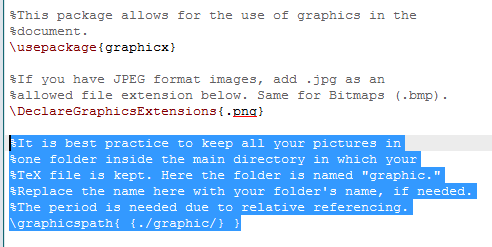
\includegraphics[scale=0.95]{GraphicDir.png}
%% 	\caption{Declaring graphics directories.}
%% \end{figure}

%% This version of the template now has a section to place any packages that you are using - see the figure below.

%% \begin{figure}[!h]
%% 	\centering
%% 	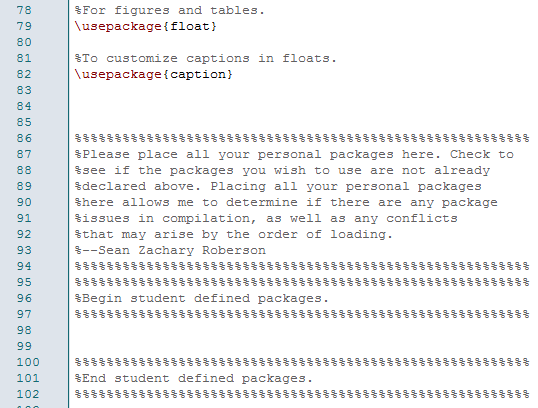
\includegraphics[scale=0.95]{CustomPackage.png}
%% 	\caption{The place to declare any packages you require that I have not already declared. This simplifies debugging.}
%% \end{figure}

%% More figures will be inserted, with some text between them.

%% \begin{figure}[!h]
%% 	\centering
%% 	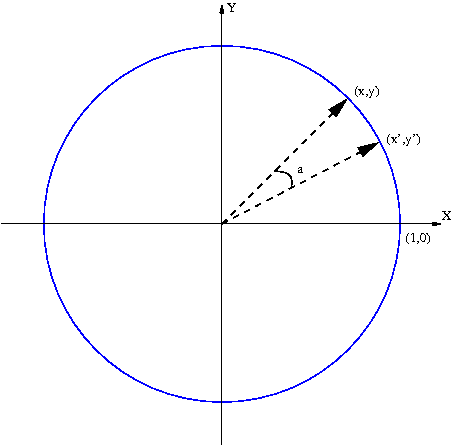
\includegraphics[scale=0.85]{CartesianCoordinate.png}
%% 	\caption{Two points on the unit circle and their corresponding position vectors.}
%% \end{figure}

%% This section has filler text. These words serve no meaning except to fill a few lines in the document. This section has filler text. These words serve no meaning except to fill a few lines in the document. This section has filler text. These words serve no meaning except to fill a few lines in the document. This section has filler text. These words serve no meaning except to fill a few lines in the document. This section has filler text. These words serve no meaning except to fill a few lines in the document. This section has filler text. These words serve no meaning except to fill a few lines in the document. This section has filler text. These words serve no meaning except to fill a few lines in the document. This section has filler text. These words serve no meaning except to fill a few lines in the document. This section has filler text. These words serve no meaning except to fill a few lines in the document. This section has filler text. These words serve no meaning except to fill a few lines in the document. This section has filler text. These words serve no meaning except to fill a few lines in the document. This section has filler text. These words serve no meaning except to fill a few lines in the document.

%% \begin{figure}[!h]
%% 	\centering
%% 	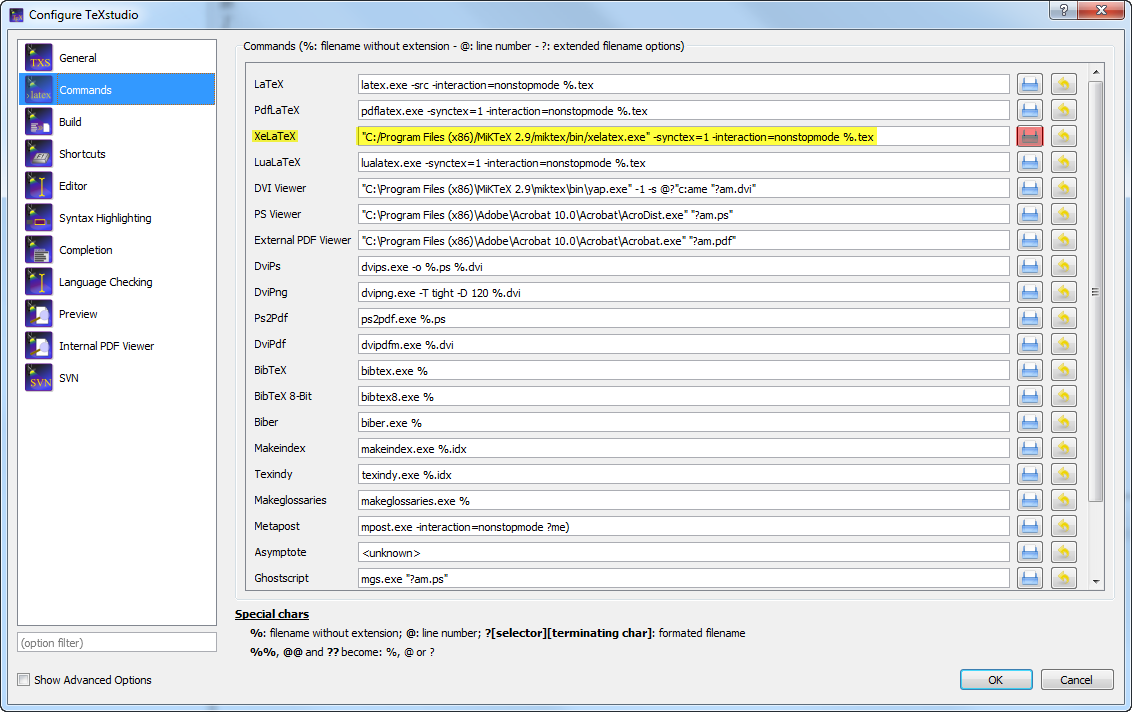
\includegraphics[width=4.25in]{CompileChange.png}
%% 	\caption{Changing the method of compilation for XeLaTeX in TeXstudio.}
%% \end{figure}

%% This section has filler text. These words serve no meaning except to fill a few lines in the document. This section has filler text. These words serve no meaning except to fill a few lines in the document. This section has filler text. These words serve no meaning except to fill a few lines in the document. This section has filler text. These words serve no meaning except to fill a few lines in the document. This section has filler text. These words serve no meaning except to fill a few lines in the document. This section has filler text. These words serve no meaning except to fill a few lines in the document. This section has filler text. These words serve no meaning except to fill a few lines in the document. This section has filler text. These words serve no meaning except to fill a few lines in the document. This section has filler text. These words serve no meaning except to fill a few lines in the document. This section has filler text. These words serve no meaning except to fill a few lines in the document. This section has filler text. These words serve no meaning except to fill a few lines in the document. This section has filler text. These words serve no meaning except to fill a few lines in the document. This section has filler text. These words serve no meaning except to fill a few lines in the document. This section has filler text. These words serve no meaning except to fill a few lines in the document. This section has filler text. These words serve no meaning except to fill a few lines in the document. This section has filler text. These words serve no meaning except to fill a few lines in the document. This section has filler text. These words serve no meaning except to fill a few lines in the document. This section has filler text. These words serve no meaning except to fill a few lines in the document.

%% \begin{figure}[!h]
%% 	\centering
%% 	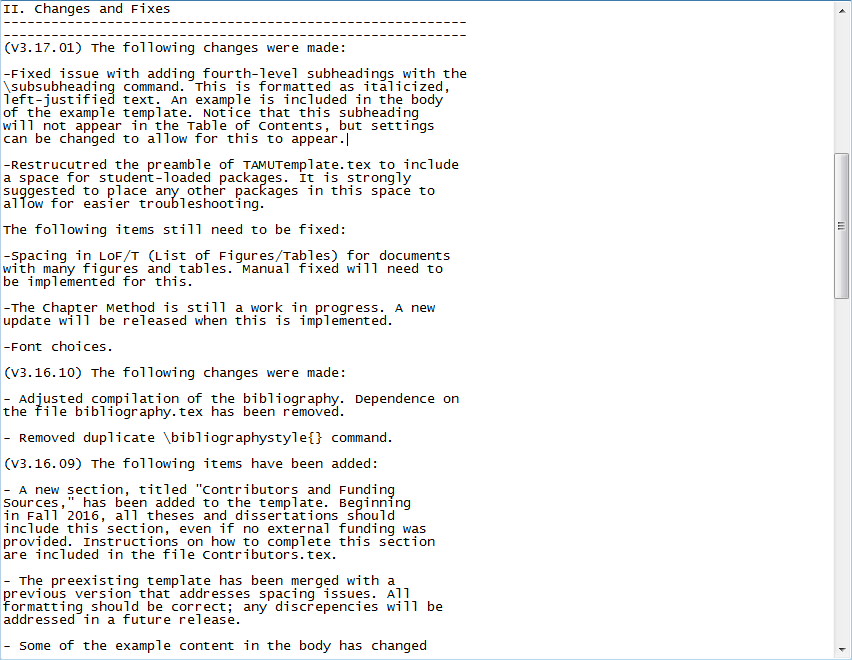
\includegraphics[width = 4.825in]{Changelog.png}
%% 	\caption{A portion of the changelog in the README for this document. This is located in the root directory.}
%% \end{figure}

%% This section has filler text. These words serve no meaning except to fill a few lines in the document. This section has filler text. These words serve no meaning except to fill a few lines in the document. This section has filler text. These words serve no meaning except to fill a few lines in the document. This section has filler text. These words serve no meaning except to fill a few lines in the document. This section has filler text. These words serve no meaning except to fill a few lines in the document. This section has filler text. These words serve no meaning except to fill a few lines in the document.

%% This section has filler text. These words serve no meaning except to fill a few lines in the document. This section has filler text. These words serve no meaning except to fill a few lines in the document. This section has filler text. These words serve no meaning except to fill a few lines in the document. This section has filler text. These words serve no meaning except to fill a few lines in the document. This section has filler text. These words serve no meaning except to fill a few lines in the document. This section has filler text. These words serve no meaning except to fill a few lines in the document. This section has filler text. These words serve no meaning except to fill a few lines in the document. This section has filler text. These words serve no meaning except to fill a few lines in the document. This section has filler text. These words serve no meaning except to fill a few lines in the document. This section has filler text. These words serve no meaning except to fill a few lines in the document. This section has filler text. These words serve no meaning except to fill a few lines in the document. This section has filler text. These words serve no meaning except to fill a few lines in the document. This section has filler text. These words serve no meaning except to fill a few lines in the document. This section has filler text. These words serve no meaning except to fill a few lines in the document. This section has filler text. These words serve no meaning except to fill a few lines in the document. This section has filler text. These words serve no meaning except to fill a few lines in the document. This section has filler text. These words serve no meaning except to fill a few lines in the document. This section has filler text. These words serve no meaning except to fill a few lines in the document.

%% \section{Challenges}
%% Section here is to test toc display only.

%% \section{Further Study}
%% Section here is to test toc display only.



%The next line is the format for inserting new sections.
%Replace the name "newsection"  with the name of your
%new section file.
%\include{data/newsection}

%fix spacing in bibliography, if any...
%%%%%%%%%%%%%%%%%%%%%%%%%%%%%%%%%%%%%%%%%%%%%%%%%%%%%%%%%%%%%
\let\oldbibitem\bibitem
\renewcommand{\bibitem}{\setlength{\itemsep}{0pt}\oldbibitem}
%%%%%%%%%%%%%%%%%%%%%%%%%%%%%%%%%%%%%%%%%%%%%%%%%%%%%%%%%%%%%%%
%The bibliography style declared is the IEEE format. If
%you require a different style, see the document
%bibstyles.pdf included in this package. This file,
%hosted by the University of Vienna, shows several
%bibliography styles and examples of in-text citation
%and a references page.
\bibliographystyle{ieeetr}

\phantomsection
\addcontentsline{toc}{chapter}{REFERENCES}

\renewcommand{\bibname}{{\normalsize\rm REFERENCES}}

%This file is a .bib database that contains the sources.
%This removes the dependency on the previous file
%bibliography.tex.
\bibliography{data/myReference}




%This next line includes appendices. The file
%appendix.tex contains commands pointing to
%the appendix files; be sure to change these
%pointers if you end up changing the filenames.
%Leave this commented if you will not need
%appendix material.
%%%%%%%%%%%%%%%%%%%%%%%%%%%%%%%%%%%%%%%%%%%%%%%%%%%%
%
%  New template code for TAMU Theses and Dissertations starting Fall 2016.  
%
%
%  Author: Sean Zachary Roberson
%  Version 3.17.09
%  Last Updated: 9/21/2017
%
%%%%%%%%%%%%%%%%%%%%%%%%%%%%%%%%%%%%%%%%%%%%%%%%%%%

\begin{appendices}
\titleformat{\chapter}{\centering\normalsize}{APPENDIX \thechapter}{0em}{\vskip .5\baselineskip\centering}
\renewcommand{\appendixname}{APPENDIX}

%%%%%%%%%%%%%%%%%%%%%%%%%%%%%%%%%%%%%%%%%%%%%%%%%%%
%
%  New template code for TAMU Theses and Dissertations starting Fall 2016.
%
%
%  Author: Sean Zachary Roberson 
%	 Version 3.16.09
%  Last updated 9/12/2016
%
%%%%%%%%%%%%%%%%%%%%%%%%%%%%%%%%%%%%%%%%%%%%%%%%%%%

%%%%%%%%%%%%%%%%%%%%%%%%%%%%%%%%%%%%%%%%%%%%%%%%%%%%%%%%%%%%%%%%%%%%%%
%%                           APPENDIX A 
%%%%%%%%%%%%%%%%%%%%%%%%%%%%%%%%%%%%%%%%%%%%%%%%%%%%%%%%%%%%%%%%%%%%%

\phantomsection

\chapter{\uppercase{First Appendix}}

Text for the Appendix follows.

\begin{figure}[h]
\centering
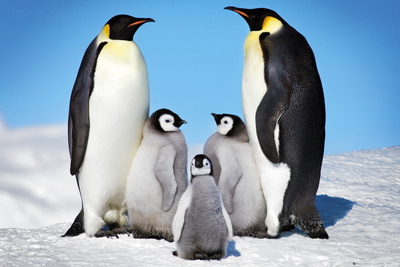
\includegraphics[scale=.50]{figures/Penguins.jpg}
\caption{TAMU figure}
\label{fig:tamu-fig5}
\end{figure}

%%%%%%%%%%%%%%%%%%%%%%%%%%%%%%%%%%%%%%%%%%%%%%%%%%%
%
%  New template code for TAMU Theses and Dissertations starting Fall 2016.
%
%
%  Author: Sean Zachary Roberson 
%	 Version 3.16.09 
%  Last updated 9/12/2016
%
%%%%%%%%%%%%%%%%%%%%%%%%%%%%%%%%%%%%%%%%%%%%%%%%%%%

%%%%%%%%%%%%%%%%%%%%%%%%%%%%%%%%%%%%%%%%%%%%%%%%%%%%%%%%%%%%%%%%%%%%%%
%%                           APPENDIX B
%%%%%%%%%%%%%%%%%%%%%%%%%%%%%%%%%%%%%%%%%%%%%%%%%%%%%%%%%%%%%%%%%%%%%

\chapter{\uppercase {A Second Appendix Whose Title Is Much Longer Than The First}}

Text for the Appendix follows.

\begin{figure}[h]
\centering
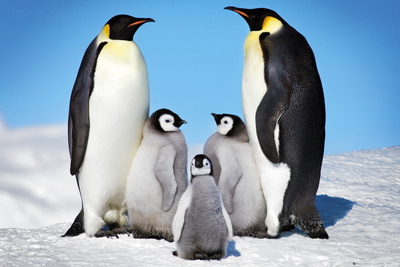
\includegraphics[scale=.50]{figures/Penguins.jpg}
\caption{Another TAMU figure.}
\label{fig:tamu-fig6}
\end{figure}

\section{Appendix Section}

\section{Second Appendix Section}


\pagebreak{}

\end{appendices}


\end{document}
